\documentclass[a4paper, 12pt]{article}

%\usepackage[cmex10]{amsmath, mathtools}
\usepackage{amsmath,amssymb,amsbsy,amsfonts,amsthm}
\usepackage{multirow}
\usepackage{bm}
\usepackage{enumerate}
\usepackage{url}
\usepackage[ruled,vlined]{algorithm2e}
\usepackage{fancyvrb}
\usepackage{yfonts}
\usepackage{dsfont}
\usepackage{calc} %    For the \widthof macro
\usepackage{xparse} %  For \NewDocumentCommand
\usepackage{wrapfig}
\usepackage{tikz}
\usepackage{lipsum}
%\input{../tikz.conf}
\usepackage{graphicx}
\usepackage{subcaption}
\usetikzlibrary{bayesnet}
\usepackage{longtable,booktabs}

%%%%%%%%%%%%%%%%%%%%
%%% Goemetry
%%%%%%%%%%%%%%%%%%%%
%\usepackage[margin=0.25in]{geometry}
\usepackage{geometry}
\geometry{
    a4paper,
 total={420pt,700pt},
 %left=20mm,
 top=20mm,
 }

\newcommand*{\lpath}{../}%

\title{Networks Properties -- Experiments}

\begin{document}

\maketitle
\tableofcontents

To illustrate our theoretical results, we evaluate the predictive performance and the ability of the models to capture homophily and preferential attachment on artificial and real networks. In the sequel, we first describe the measures used to evaluate the properties of interest and the predictive performance, then the datasets used in our experiments. Afterwards, we detail the evaluation protocol and we present the experimental results.

\section{pymake software}
All our experiments were realized with a frameworks that we developed, and open sourced, available at : https://github.com/dtrckd/pymake. This repository is in current active development in order ot populate Bayesian modelisation, and to do reproducible research. The framework currently contains Gibbs sampler for the MMSB and ILFM notably for parametric and nonparametric versions. The frameworks also aims helping the design of experiments, the use of available datasets online and working scientific library such as \emph{numpy} \footnote{http://www.numpy.org/}, \emph{scikit-learn} \footnote{http://scikit-learn.org/}, \emph{networkx} \footnote{https://networkx.github.io/} and others.

\section{Evaluation Measures}
This article focus on two properties of networks, namely the preferential attachment effect and the homophily. In this section, we present the measures used in our experiments in order to characterized these properties and to evaluate the predictive performance of the models.

\subsection{Measures for the properties}

\subsubsection{Preferential attachment}
\label{sec:experiments-burst}

The measures considered to evaluate the preferential attachment rely on a goodness of fit. Indeed, it has been reported that preferential attachment leads to networks characterized by a degree distribution with heavy tail drawn from a power law \textbf{ref?}. A graphical method, most often used to verify that the observations are consistent with this law  consists in constructing the histogram representing the degree distribution and if the plot on doubly logarithmic axes approximately falls on a straight line, then one can assume that the distribution follows a power law. Thus, the comparison of the degree distribution in the log-log scale with a linear function gives us a qualitative measure for the preferential attachment. To obtain a second evaluation of the power law hypothesis for the degree distribution, we follow the statistical framework, introduced by \cite{clauset2009power}, for discerning and quantifying power-law behavior in empirical data. This framework combines maximum-likelihood fitting methods with goodness-of-fit tests based on the Kolmogorov-Smirnov statistic. It includes the following steps:


\begin{itemize}
	\item Estimate the parameters $\alpha$ and $x_\text{min}$ of the power law model. $\alpha$ is the scaling parameter of the law and $x_\text{min}$, the lower bound for the tail,  has been fix in our experiments, to the smallest value observed in the distributions evaluated, to allow their comparisons.
	\item  Using the Kolmogorov-Smirnov (KS) statistic, compute the distance $KS_{obs}$  between the degree distribution obtained on the network with the theoretical distribution corresponding to the power law with the estimated parameters.
	\item Sample $S$ synthetic datasets from the power law with the estimated parameters. For each sample s, using the Kolmogorov-Smirnov statistic, compute the distance $KS_{s}$ between the distribution obtained on this synthetic dataset drawn from the power law with the corresponding theoretical distribution. According to  \cite{clauset2009power}, the number of samples $S$ is chosen such that $S = \frac{1}{4}\epsilon^{-2}$, with a precision  $\epsilon = 3^{-2}$. 
    \item  The p-value is defined as the fraction of  the resulting statistics $KS_s, s \in \{1,...,S\}$ obtained on the samples larger than the value $KS_{obs}$ computed on the network distribution.  
\end{itemize}

 If  p-value is large (close to 1), then the difference between the data and the model can be attributed to statistical fluctuations alone; if it is small, the model is not a plausible fit for the data and we can not conclude that there is an evidence for the preferential attachment in the network. 
\textbf{arevoir}However, as mentioned in \cite{clauset2009power} high value of the $p$-value should be considered with caution for at least two reasons. First, there may be other distribution that match the data equally or better. Second, a small number of samples of the data may lead to high p-value and reflect the fact that is hard to rule out a hypothesis in such a case.


\paragraph{Local burstiness : }
In the context of latent models, while there is no ambiguity in computing the overall degree distribution, it is less obvious for the local case. We explain here the computation of the local degree distribution for each models according to section \ref{sec:burstiness} :
\begin{itemize}
        \item for IMMSB, each network has an associated membership tensor $Z$, that indicates the membership of nodes for each  interactions. In order to draw the local degree distribution for a block $c$, we reduce the adjacency matrix in order to retain only the links that occurs inside a block $c$. The local degree distribution is thus computed on the reduce adjacency matrix defines as follows $Y^c =\{ y_{ij}^c=1 \ \textrm{if}\ y_{ij}=1 , z_{i\rightarrow j}=c, z_{i\leftarrow j}=c\}$.
        \item for ILFM, each node is associated with a fix feature vector; the local degree distribution for the block $c$ is obtain by taking only the contribution of the features $c$ on the adjacency matrix. Thus, the local degree degree distribution is computed on the reduce adjacency matrix defined by $Y^c =\{ y_{ij}^c=1 \ \textrm{if}\ y_{ij}=1 , f_{ic}=1, f_{jc}=1\}$
\end{itemize}

\subsubsection{Homophily}

For the homophily property, defined in section \ref{sec:homophily}, we rely on two different measures:

\begin{itemize}
    \item  Pearson correlation coefficient between the probability of having a link $P(y_{ij}=1)$  and the natural or latent similarity ($s_n(i,j)$ and $s_l(i,j)$) for all pairs of vertices $(i,j) \in E^2 $. 
    \item  Means and variances of the similarity ($s_n(i,j)$ and $s_l(i,j)$) computed on the linked and non-linked pairs of nodes.
\end{itemize}

\subsection{Prediction performance evaluation}
The prediction problem is equivalent to a binary prediction problem in two classes since it consists to decide for each pair of nodes if there is an edge or not between them. 
Thus, the performance of the models can be evaluated with usual measures:

\begin{itemize}

\item Precision/Recall/$F_1$ :  The local precision, recall and $F_1$ scores concern the links predicted as an edge.  The global (precision), denoted global in the tables, refers to the accuracy of the model. 
\item AUC-ROC : Receiver operating characteristic curves allow also to graphically compare the  models on each dataset.
\end{itemize}

\section{Training Datasets}

In our experiments, we consider four artificial networks and four real networks.  Main topological characteristics of these networks are summarized in Table \ref{table:networks_measures} and we describe those networks in the sequel.

\begin{table}[h] 
	\centering
	\caption{Characteristics of artificial and real networks.}
	%\resizebox{\textwidth}{!}{  
    \begin{tabular}{lrrr}
        \hline
        \textbf{Networks} &   nodes &   edges &   density \\
        \hline
        Network 1 &    1000 &    3507 &     0.007 \\
        Network 2 &    1000 &    3000 &     0.006 \\
        Network 3 &    1000 &    6000 &     0.012 \\
        Network 4 &    1000 &   31000 &     0.062 \\
        Manufacturing &     167 &    5950 &     0.215 \\
        UC Irvine     &    1899 &   22195 &     0.006 \\
        Blogs         &    1490 &   20512 &     0.009 \\
        Emaileu       &    1004 &   25899 &     0.026 \\
        Protein       &    2114 &    4317 &     0.002 \\
    \hline
    \end{tabular}
	\label{table:networks_measures}
\end{table}



\subsection{Artificial networks}

The artificial networks have been generated with DANC-Generator \cite{largeron2015}. This generator has been chosen because it allows to build an attributed graph having a community structure  and  the known properties of real-world networks such as preferential attachment and homophily.
Moreover, by modifying the parameters, these properties can be weakened. Finally, DANC-Generator is available under the terms of the GNU Public License and the parameters can be shared for experiments reproducibility.

Four artificial networks (Network1, ..., Network4) have been generated. Their adjacency matrices and global degree distributions are presented in Figure \ref{fig:synt_graph}. Table \ref{table:synt_graph} gives the resulting $p$-value of the KS test as well as the  values estimated for the parameters  $\alpha$ and $x_\text{min}$,  and  the number $n_{tail}$ of observations in the distribution such as $x \geq x_\text{min}$ . For each network, Figure \ref{fig:synt_graph_local} represents the local degree distribution associated to each \emph{ground truth} community and Table \ref{table:synt_graph_local} reports the KS results in the local case. The inner degree distribution (edges inside a community) and outer degree distribution (edges between community) are plotted separately.

Each network presents a different affinity to preferential attachment and homophily.
Indeed, As shown Figure \ref{fig:synt_graph}, Network1 and Network2, and to a lesser extend, Network3 verify preferential attachment whereas it is not the case for Network4. The results of the KS test given in Table \ref{table:synt_graph} confirm this analysis since the $p$-value is very high for Network1 and Network2, respectively equals to 1 and 0.99 but it decreases for Network3 and is equal 0 for Network4.
Concerning the local preferential attachment, that can be evaluated on these artificial networks where the ground truth communities are provided by the generator, the local degree distributions per class are given in Figure \ref{fig:synt_graph_local} and the average results (and variances) for the p-value computed over the classes are reported in Table \ref{table:synt_graph_local}. They show that the local preferential attachment is verified in the two first networks and in a lesser extend for the  last ones. In particularly, the high variance of the $p$-value for Network3 and Network4 indicates that the property varies among the classes.


\begin{figure}[h]
        \begin{minipage}{0.24\textwidth}
            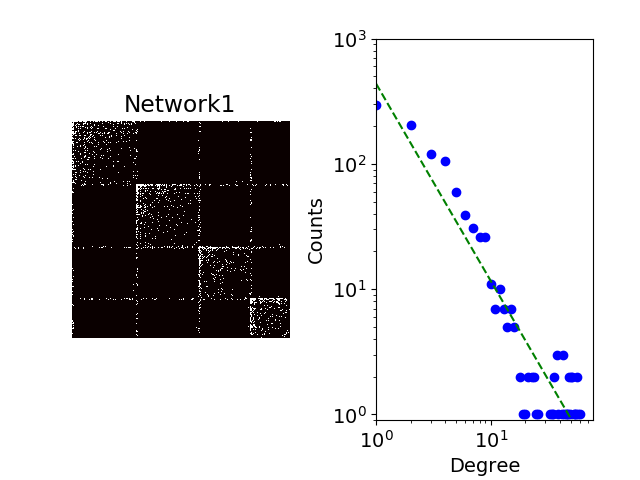
\includegraphics[width=\textwidth]{img/corpus/network1_dd}
        \end{minipage}
        \begin{minipage}{0.24\textwidth}
            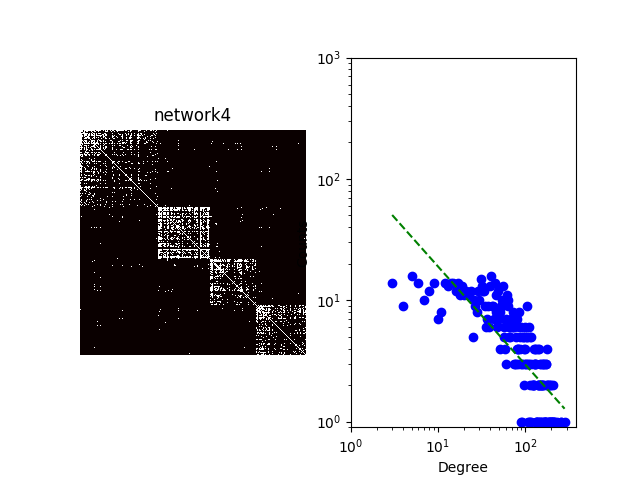
\includegraphics[width=\textwidth]{img/corpus/network4_dd}
        \end{minipage}
        \vskip\baselineskip
        \begin{minipage}{0.24\textwidth}
            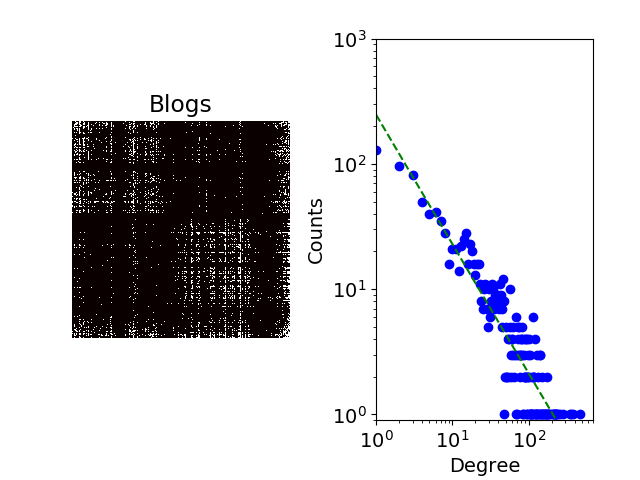
\includegraphics[width=\textwidth]{img/corpus/blogs_dd}
        \end{minipage}
        \begin{minipage}{0.24\textwidth}
            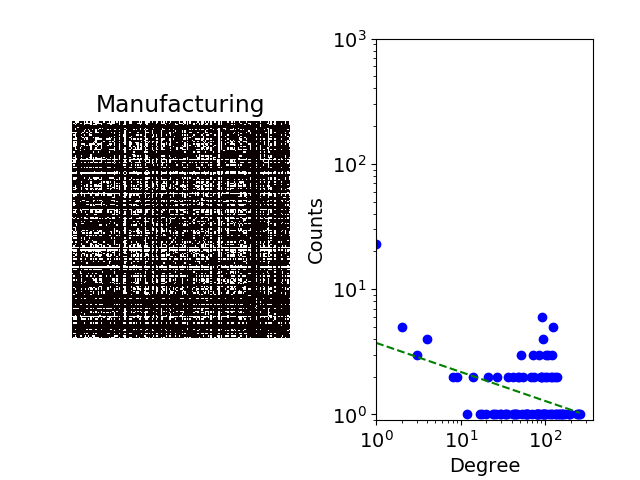
\includegraphics[width=\textwidth]{img/corpus/manufacturing_dd}
        \end{minipage}
	\caption{Adjacency matrices (left) and global degree distributions (right) for the networks datasets.}
	\label{fig:corpuses}
\end{figure}


\begin{figure}[h]
        \begin{minipage}{0.24\textwidth}
            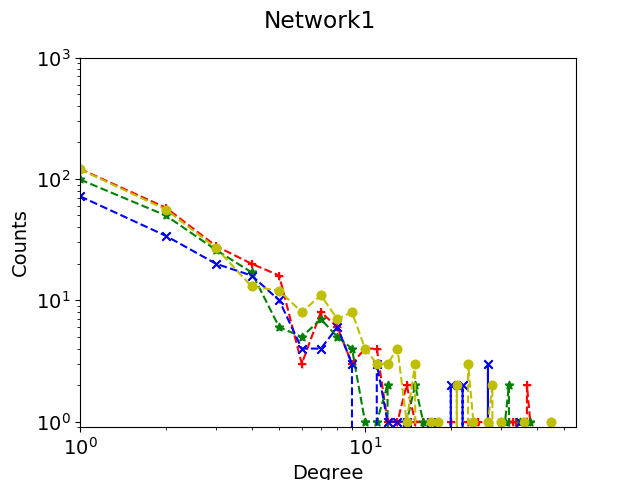
\includegraphics[width=\textwidth]{img/corpus/network1_1}
        \end{minipage}
        \begin{minipage}{0.24\textwidth}
            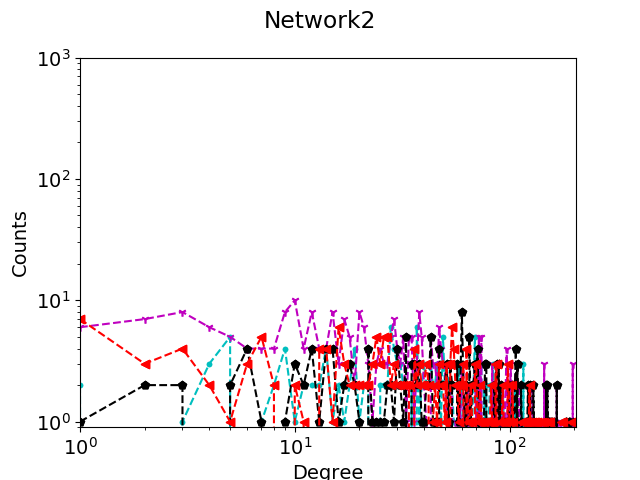
\includegraphics[width=\textwidth]{img/corpus/network2_1}
        \end{minipage}
        \vskip\baselineskip
        \begin{minipage}{0.24\textwidth}
            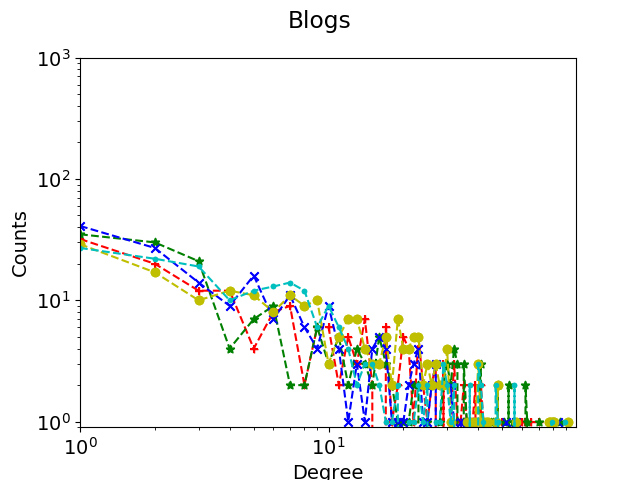
\includegraphics[width=\textwidth]{img/corpus/blogs_1}
        \end{minipage}
        \begin{minipage}{0.24\textwidth}
            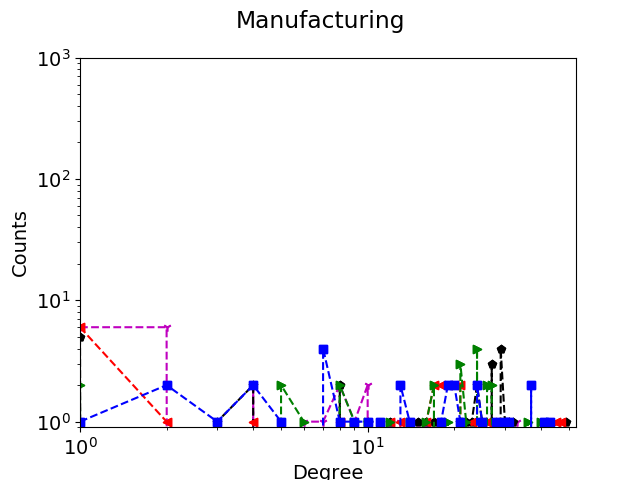
\includegraphics[width=\textwidth]{img/corpus/manufacturing_1}
        \end{minipage}
        \caption {Local degree distributions for the four networks datasets. Inner(left) and outer(right) degree are separated. For Network1 and Network2 the classes come from ground-truth. For Blogs and Manufacturing we use classes find by a Louvain algorithms.} 
	\label{fig:synt_graph_local}
\end{figure}


\begin{table}[h]
\caption{Power law goodness of fit results for the global preferential attachment in artificial networks.}
\centering
  \begin{tabular}{lrrrr}
  	\hline
  	&   pvalue &   alpha &   x\_min &   n\_tail \\
  	\hline
  	Network 1 &    1.000 &   2.424 &       3 &     1000 \\
  	Network 2 &    0.993 &   2.897 &       3 &     1000 \\
  	Network 3 &    0.765 &   1.758 &       3 &     1000 \\
  	Network 4 &    0.000 &   1.354 &       3 &     1000 \\
  	\hline
  \end{tabular}
\label{table:synt_graph}
\end{table}

\begin{table}[h]
\caption{Power law goodness of fit results for the local preferential attachment in artificial networks.}
\centering
    \begin{tabular}{lllll}
    \hline
    & pvalue          & alpha           & x\_min        & n\_tail           \\
    \hline
    Network1 & 0.9 $\pm$ 0.07  & 2.7 $\pm$ 0.1 & 1.8 $\pm$ 0.9 & 154.4 $\pm$ 83.9 \\
    Network2 & 0.9 $\pm$ 0.008 & 3.0 $\pm$ 1.2  & 1.8 $\pm$ 0.9 & 170.9 $\pm$ 66.4  \\
    Network3 & 0.8 $\pm$ 0.26 & 7.0 $\pm$ 5.8 & 1.8 $\pm$ 0.9 & 136.3 $\pm$ 94.0 \\
    Network4 & 0.6 $\pm$ 0.49    & 1.5 $\pm$ 0.1 & 1.8 $\pm$ 0.9 & 204.7 $\pm$ 53.0 \\
    \hline
    \end{tabular}


    %% THE GOOD ONE !
%    __IMMSB__    pvalue             alpha              x_min          n_tail
%    -----------  -----------------  -----------------  -------------  ------------------
%    Network 1    1.0 $\pm$ 0.0      2.394 $\pm$ 0.509  1.0 $\pm$ 0.0  154.4 $\pm$ 83.995
%    Network 2    1.0 $\pm$ 0.0      2.231 $\pm$ 0.225  1.0 $\pm$ 0.0  170.9 $\pm$ 66.44
%    Network 3    0.987 $\pm$ 0.009  1.398 $\pm$ 0.008  1.0 $\pm$ 0.0  250.0 $\pm$ 22.034
%    Network 4    0.6 $\pm$ 0.49     1.538 $\pm$ 0.251  1.0 $\pm$ 0.0  204.7 $\pm$ 53.008


\label{table:synt_graph_local}
\end{table}

\subsection{Real networks}

We evaluated also the models on five real networks.
The first one, denoted UC Irvine \footnote{available at:}, is built from a online community of 1899 students from the University of California. Each node corresponds to a user and a   directed edge represents a sent message.
The second one, denoted Manufacturing \footnote{available at:}, is an internal email communication network between employees of a mid-sized manufacturing company. Each vertex is associated  to an employee and an oriented link represents like previously a sent email.

The adjacency matrices and global degree distributions are presented in Figure \ref{fig:real_graph}. The goodness of fit based on the KS test, used as a reference for the global preferential attachment effect, is reported in Table \ref{table:real_graph}. According to Figure \ref{fig:real_graph} as well as Table \ref{table:real_graph}, it appears that the preferential attachment property is verified in UC Irvine, with a p-value equals to 0.989, and not in Manufacturing where the p-value is null. As the ground truth is not available for these networks, the local preferential attachment can not be verified.


%\begin{figure}[h]
%        \centering
%        \begin{subfigure}[b]{0.400\textwidth}
%            \centering
%            \includegraphics[scale=0.38]{img/corpus/fb_uc.png}
%            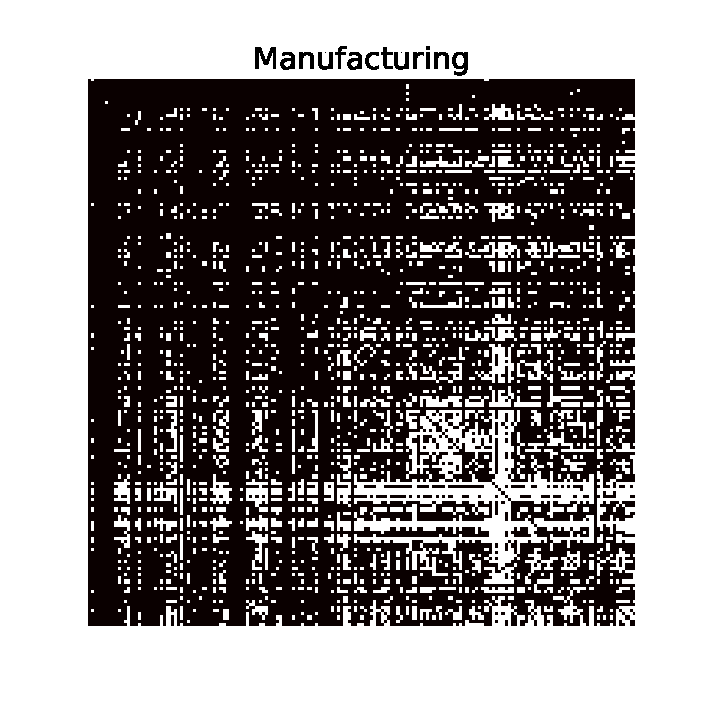
\includegraphics[scale=0.38]{img/corpus/manufacturing.png}
%            \caption {{\small Adjacency matrix}}    
%            \label{fig:mean and std of net14}
%        \end{subfigure}
%        %\hfill
%        \quad
%        \begin{subfigure}[b]{0.400\textwidth}  
%            \centering 
%            \includegraphics[scale=0.42]{img/corpus/fb_uc_d.png}
%            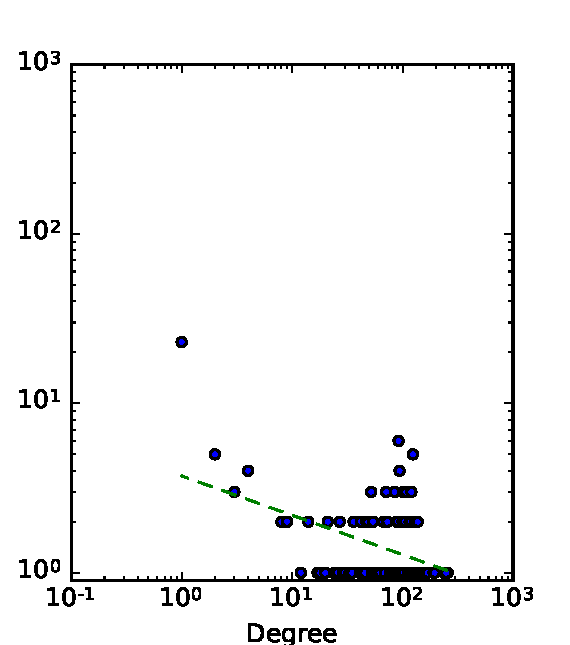
\includegraphics[scale=0.42]{img/corpus/manufacturing_d.png}
%            \caption {{\small Overall degree distributions}}    
%            \label{fig:mean and std of net24}
%        \end{subfigure}
%       \caption{Adjacency matrices (left) and global degree distributions (right) for the real networks.}
%    \label{fig:real_graph}
%\end{figure}

\begin{figure}[h]
        \centering
        \begin{subfigure}[b]{0.480\textwidth}
            \centering
            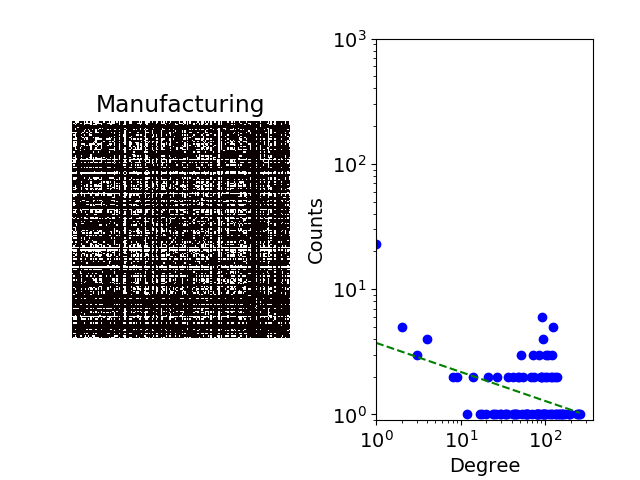
\includegraphics[width=\textwidth]{img/corpus/manufacturing_dd}
            \caption {{\small Manufacturing}}    
            \label{fig:mean and std of net14}
        \end{subfigure}
        \hfill
        \begin{subfigure}[b]{0.480\textwidth}  
            \centering 
            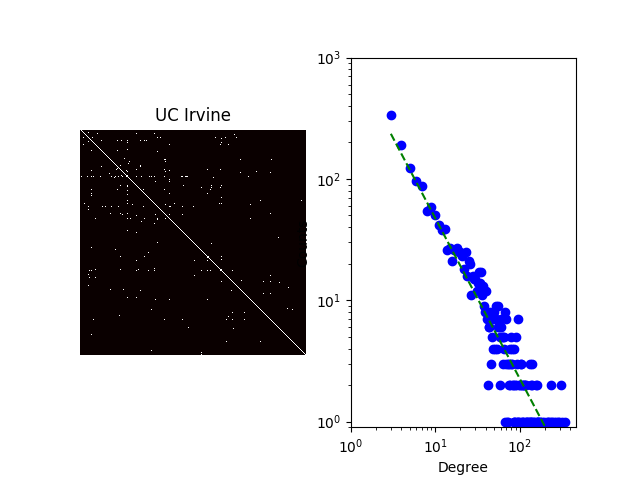
\includegraphics[width=\textwidth]{img/corpus/fb_uc_dd}
            \caption {{\small UC Irvine}}    
            \label{fig:mean and std of net24}
        \end{subfigure}
        \vskip\baselineskip
        \begin{subfigure}[b]{0.480\textwidth}   
            \centering 
            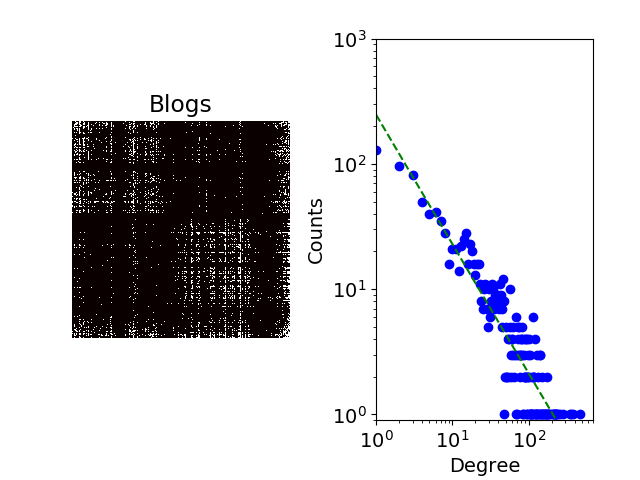
\includegraphics[width=\textwidth]{img/corpus/blogs_dd}
            \caption{{\small Blogs}}    
            \label{fig:mean and std of net34}
        \end{subfigure}
        \quad
        \begin{subfigure}[b]{0.480\textwidth}   
            \centering 
            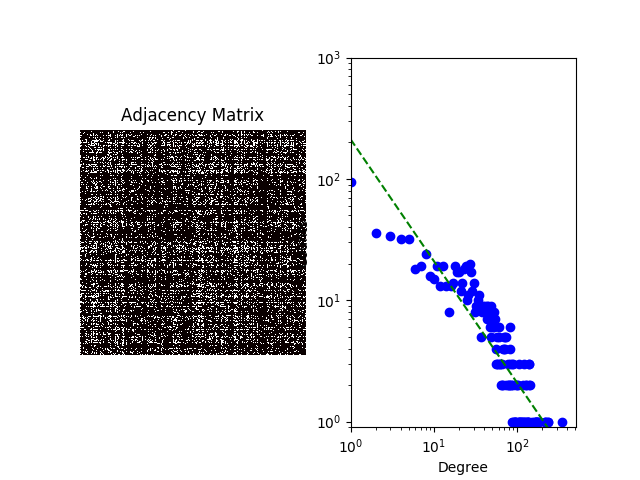
\includegraphics[width=\textwidth]{img/corpus/emaileu_dd}
            \caption{{\small Emaileu}}    
            \label{fig:mean and std of net44}
        \end{subfigure}
        \begin{subfigure}[b]{0.480\textwidth}   
            \centering 
            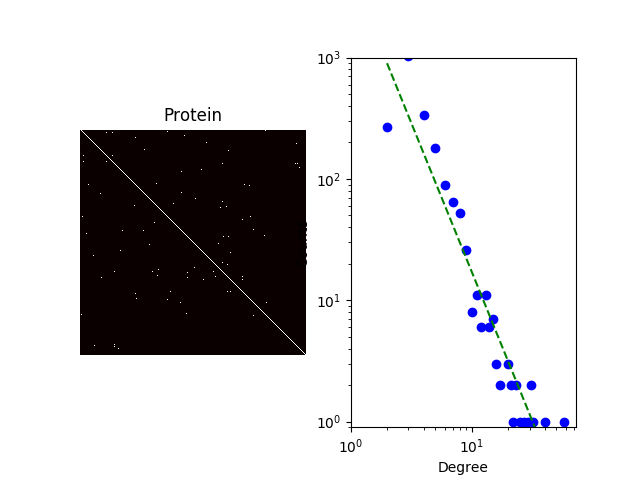
\includegraphics[width=\textwidth]{img/corpus/propro_dd}
            \caption{{\small Protein}}    
            \label{fig:mean and std of net44}
        \end{subfigure}
        %\begin{subfigure}[b]{0.480\textwidth}   
        %    \centering 
        %    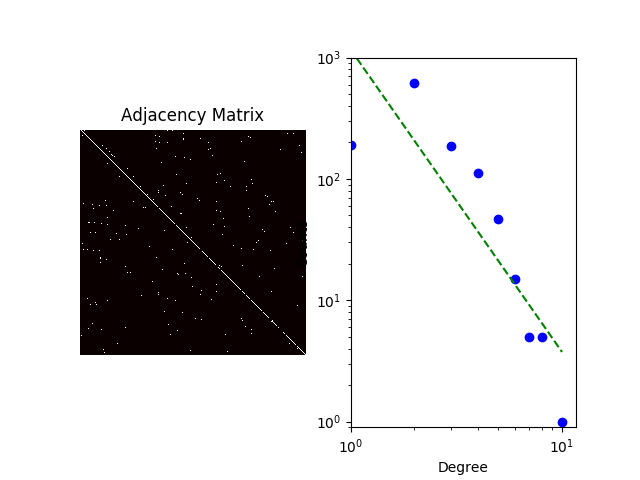
\includegraphics[width=\textwidth]{img/corpus/euroroad_dd}
        %    \caption{{\small Euroroad}}    
        %    \label{fig:mean and std of net44}
        %\end{subfigure}
	\caption{Adjacency matrices (left) and global degree distributions (right) for the real networks.}
    \label{fig:real_graph}
\end{figure}


\begin{table}
\caption{Power law goodness of fit results for the global degree attachment in real networks.}
\centering
\begin{tabular}{lrrrr}
	\hline
	&   pvalue &   alpha &   x\_min &   n\_tail \\
	\hline
	Manufacturing &    0.000 &   1.434 &       3 &      167 \\
	UC Irvine     &    0.993 &   1.787 &       3 &     1899 \\
	Blogs         &    1.000 &   1.526 &       2 &     1490 \\
	Emaileu       &    0.000 &   1.392 &       2 &     1004 \\
	Protein       &    1.000 &   2.190 &       2 &     2114 \\
	\hline
\end{tabular}

\label{table:real_graph}
\end{table}



\section{$M_e$ -- Model fitted}

For each dataset described earlier, we run a MCMC inference consisting of 200 iterations to learn the posterior distribution for the IMMSB and ILFM  models described in section \ref{sec:models}. For IMMSB, the concentration parameters of HDP were optimized according to  \cite{HDP} using vague gamma priors $\alpha_0 \sim \text{Gamma}(1,1)$ and $\gamma \sim \text{Gamma}(1,1)$. The parameters for the matrix weights were fixed to $\lambda_0=\lambda_1=0.1$. For ILFM, the IBP hyper-parameter was fixed to $\alpha=0.5$ and the weights hyper-parameter to $\sigma_w = 1$. 

The inference procedure was run with these settings for the four datasets networks previously described.

All our experimental platform is available online \footnote{https://github.com/dtrckd/pymake}. It is an ongoing development in order to provide a flexible way to design and run experiments and make data analysis.

\subsection{Preferential attachment}

In order to evaluate the preferential attachment (local and global), we used the models to generate full networks. The procedure  is similar than those explained in section \ref{sec:mgmg}. Thus, given the model parameters $\mathcal{M}_e = \{F ,\Phi\}$ learned from an initial network, we generate a set of 20 networks, noted with an asterisk and corresponding to this original network  and, the results presented in the sequel are averaged on this set and given with the standard deviation. 

% Global
The global degree distribution of the  networks generated with  IMMSB and ILFM are respectively presented in Figures \ref{fig:me_fit_gburst_mmsb} and \ref{fig:me_fit_gburst_ibp}. Table \ref{table:global_gof} provides  the corresponding goodness of fit evaluation.
IMMSB and ILFM pass the goodness of fit test for Network1*, Network2* and UC Irvine* with high p-value (0.907 or 1) but that is not the case  for the three other networks (Network3*, Network4* and Manufacturing*) with a p-value near or equals to zero. This shows that even if the models IMMSB and ILFM  are neutral with respect to global preferential attachment, they are able to generate  networks having the property,  when this property is strongly verified in the original network used to learn the parameters.
\textbf{ARV} When the global preferential attachment is less strong, as for Network3, we can noticed if we consider the tail of the generated distributions, ILFM appears to have straight tail than ILFM.


\begin{figure}[h]
        \centering
        \begin{subfigure}[b]{0.300\textwidth}
            \centering
            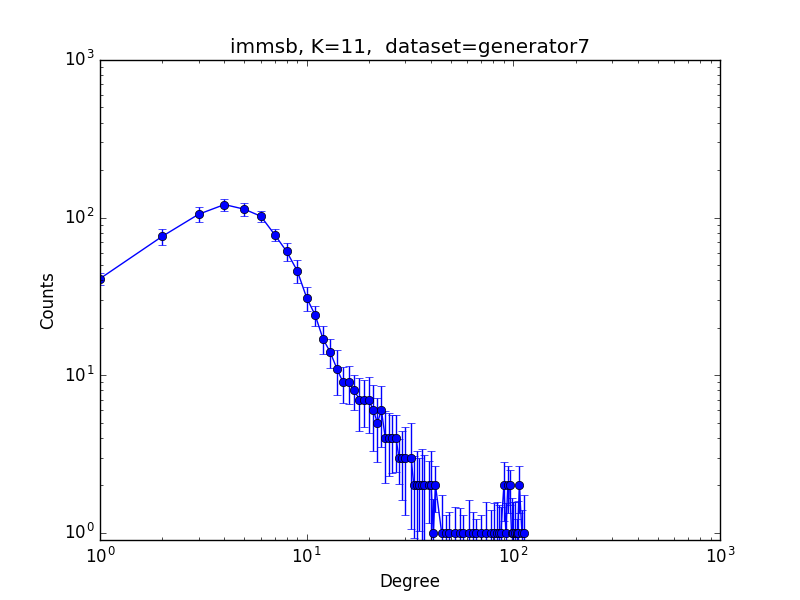
\includegraphics[width=\textwidth]{img/expe/1_mmsb/figure_1}
            \label{fig:mean and std of net14}
            \caption {{\small Network1}}    
        \end{subfigure}
        \begin{subfigure}[b]{0.300\textwidth}
            \centering
            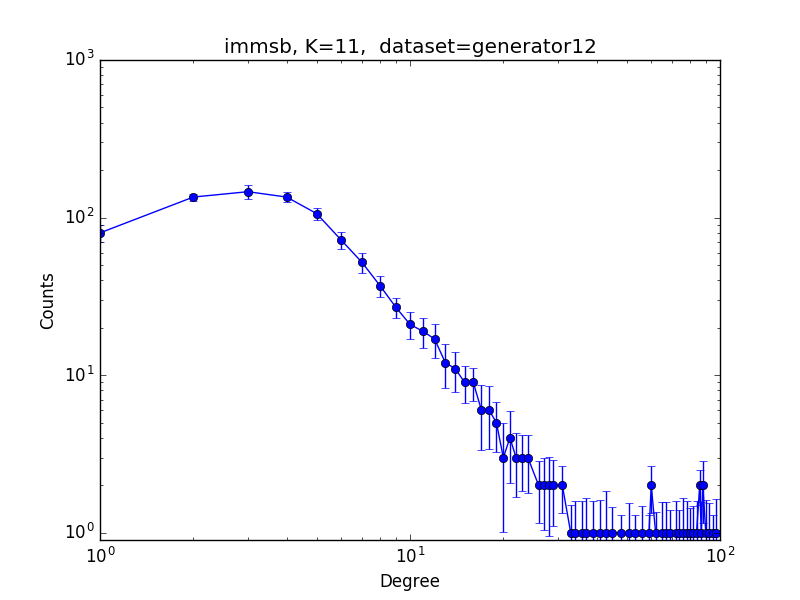
\includegraphics[width=\textwidth]{img/expe/2_mmsb/figure_1}
            \label{fig:mean and std of net14}
            \caption {{\small Network2}}    
        \end{subfigure}
        \begin{subfigure}[b]{0.300\textwidth}
            \centering
            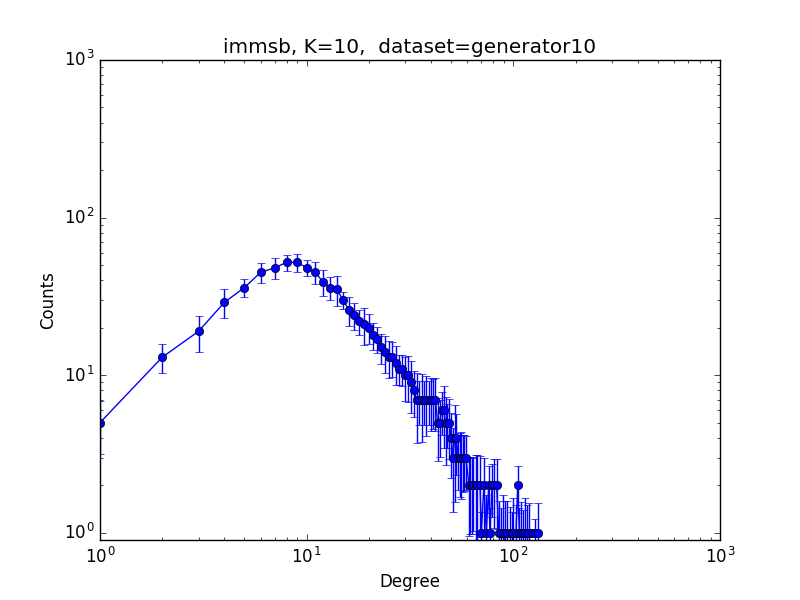
\includegraphics[width=\textwidth]{img/expe/3_mmsb/figure_1}
            \label{fig:mean and std of net14}
            \caption {{\small Network3}}    
        \end{subfigure}
        \begin{subfigure}[b]{0.300\textwidth}
            \centering
            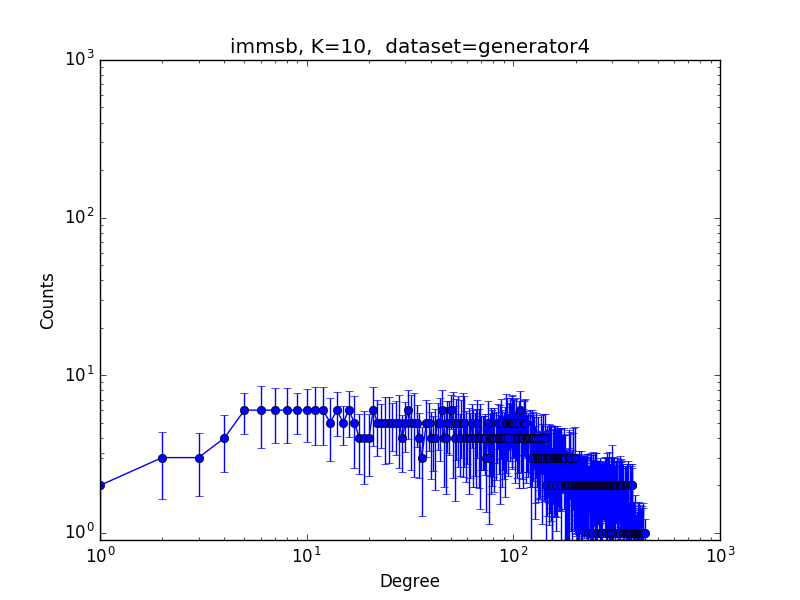
\includegraphics[width=\textwidth]{img/expe/4_mmsb/figure_1}
            \label{fig:mean and std of net14}
            \caption {{\small Network4}}    
        \end{subfigure}
        \begin{subfigure}[b]{0.300\textwidth}
            \centering
            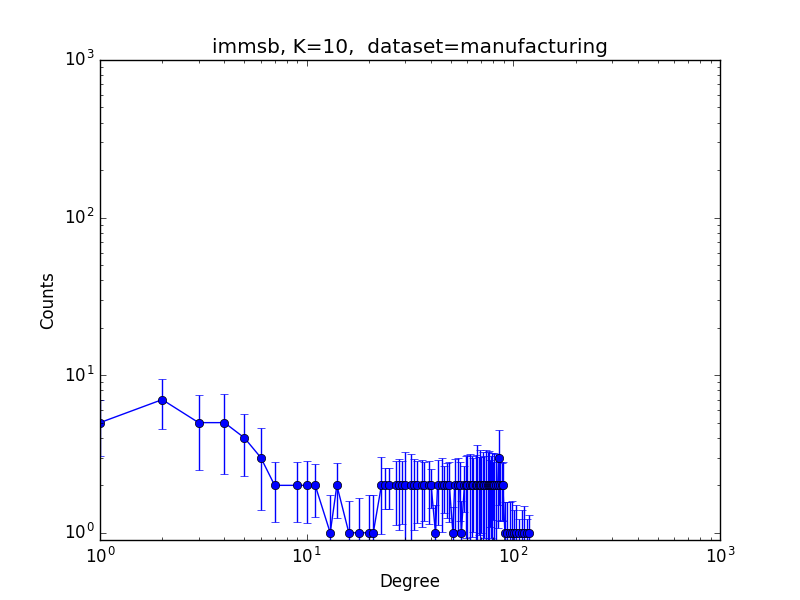
\includegraphics[width=\textwidth]{img/expe/5_mmsb/figure_1}
            \label{fig:mean and std of net14}
            \caption {{\small Manufacturing}}    
        \end{subfigure}
        \begin{subfigure}[b]{0.300\textwidth}
            \centering
            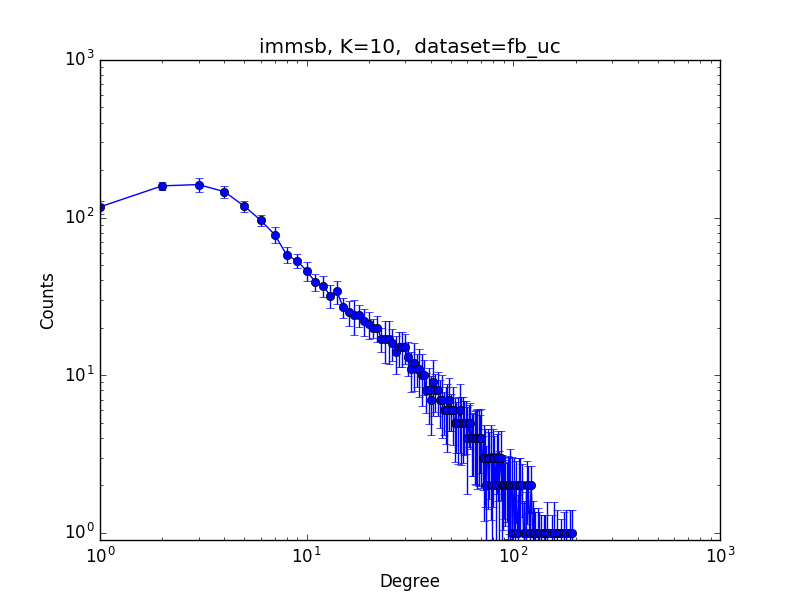
\includegraphics[width=\textwidth]{img/expe/6_mmsb/figure_1}
            \caption {{\small UC Irvine}}    
            \label{fig:mean and std of net14}
        \end{subfigure}
        %\quad
        %\hfill
        \caption{IMMSB global degree distribution in the $M_e$ settings. } 
        \label{fig:me_fit_gburst_mmsb}
\end{figure}


\begin{figure}[h]
        \centering
        \begin{subfigure}[b]{0.300\textwidth}
            \centering
            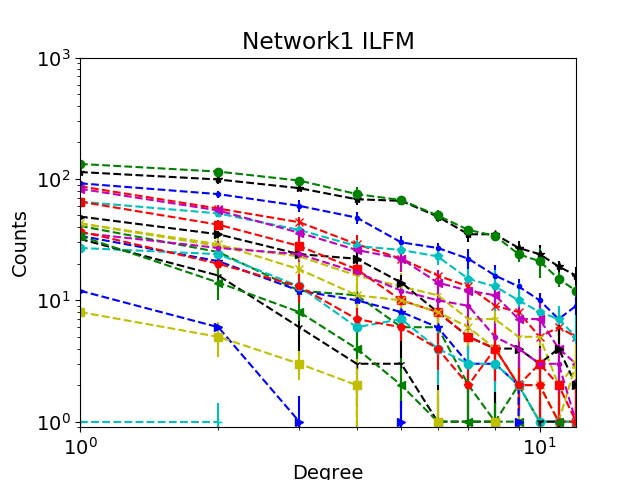
\includegraphics[width=\textwidth]{\lpath/img/corpus/ilfm_network1_0}
            \caption {{\small Network1}}    
        \end{subfigure}
        \begin{subfigure}[b]{0.300\textwidth}
            \centering
            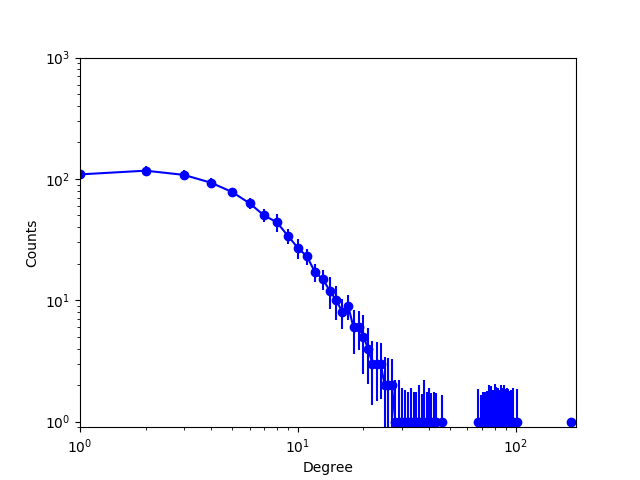
\includegraphics[width=\textwidth]{\lpath/img/corpus/ilfm_network2_0}
            \caption {{\small Network2}}    
        \end{subfigure}
        \begin{subfigure}[b]{0.300\textwidth}
            \centering
            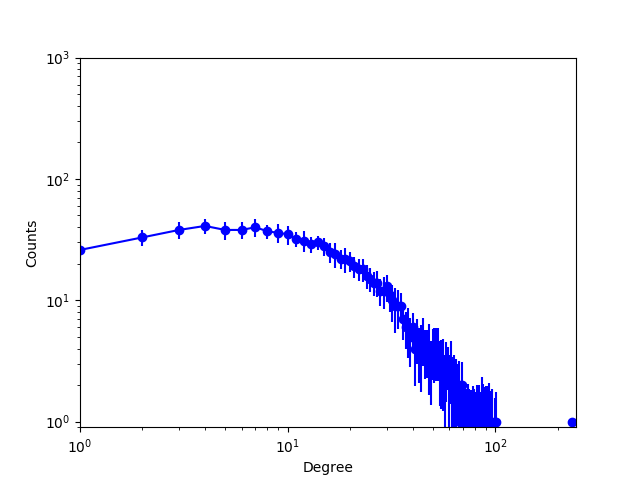
\includegraphics[width=\textwidth]{\lpath/img/corpus/ilfm_network3_0}
            \caption {{\small Network3}}    
        \end{subfigure}
        \begin{subfigure}[b]{0.300\textwidth}
            \centering
            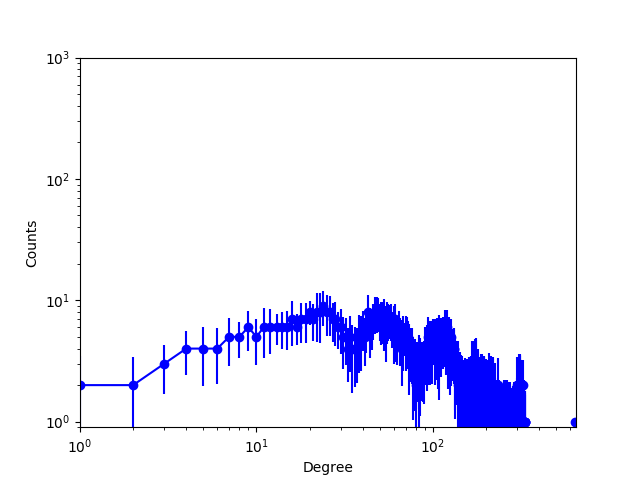
\includegraphics[width=\textwidth]{\lpath/img/corpus/ilfm_network4_0}
            \caption {{\small Network4}}    
        \end{subfigure}
        \begin{subfigure}[b]{0.300\textwidth}
            \centering
            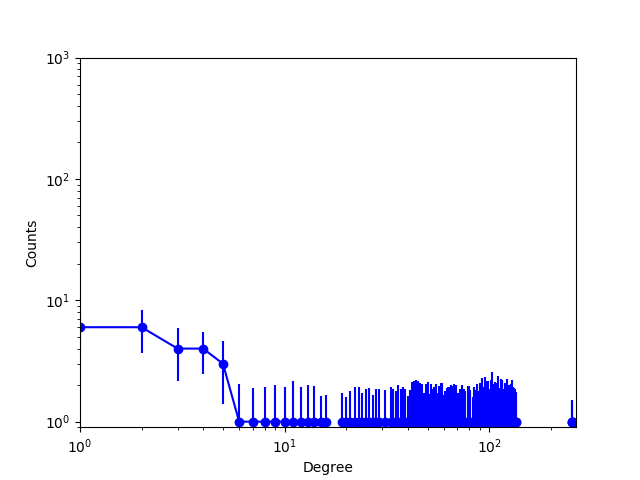
\includegraphics[width=\textwidth]{\lpath/img/corpus/ilfm_manufacturing_0}
            \caption {{\small Manufacturing}}    
        \end{subfigure}
        \begin{subfigure}[b]{0.300\textwidth}
            \centering
            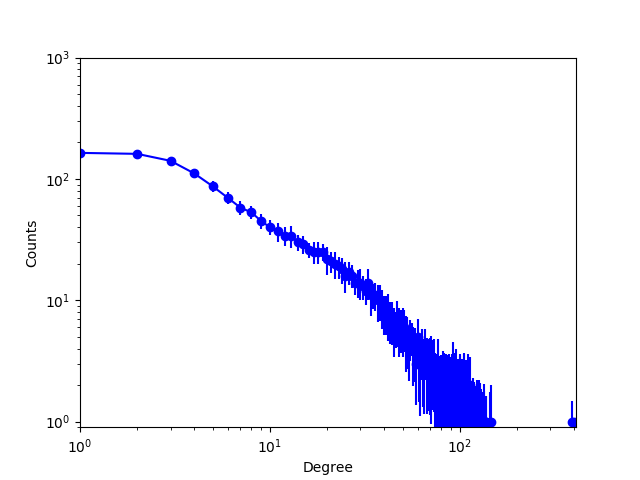
\includegraphics[width=\textwidth]{\lpath/img/corpus/ilfm_ucirvine_0}
            \caption {{\small UC Irvine}}    
            \label{fig:mean and std of net14}
        \end{subfigure}
        \begin{subfigure}[b]{0.300\textwidth}
            \centering
            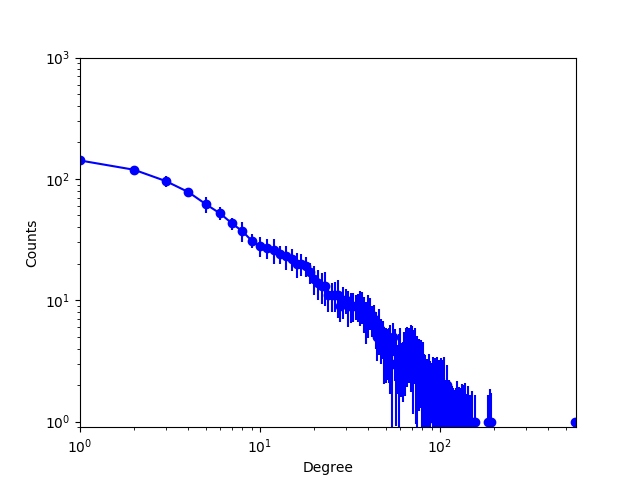
\includegraphics[width=\textwidth]{\lpath/img/corpus/ilfm_blogs_0}
            \caption {{\small Blogs}}    
            \label{fig:mean and std of net14}
        \end{subfigure}
        \begin{subfigure}[b]{0.300\textwidth}
            \centering
            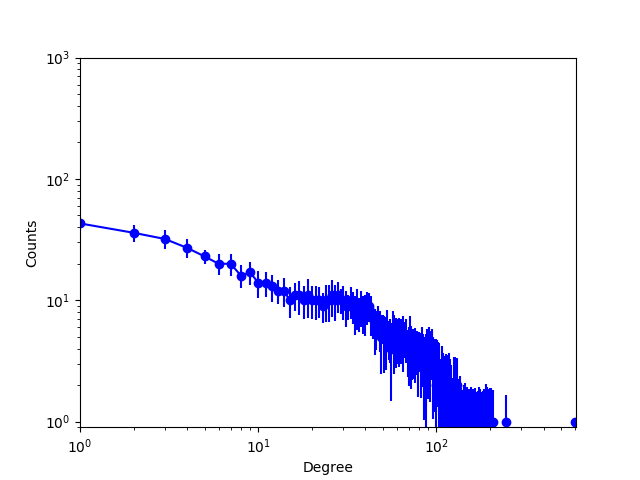
\includegraphics[width=\textwidth]{\lpath/img/corpus/ilfm_emaileu_0}
            \caption {{\small Email Europe}}    
            \label{fig:mean and std of net14}
        \end{subfigure}
        \begin{subfigure}[b]{0.300\textwidth}
            \centering
            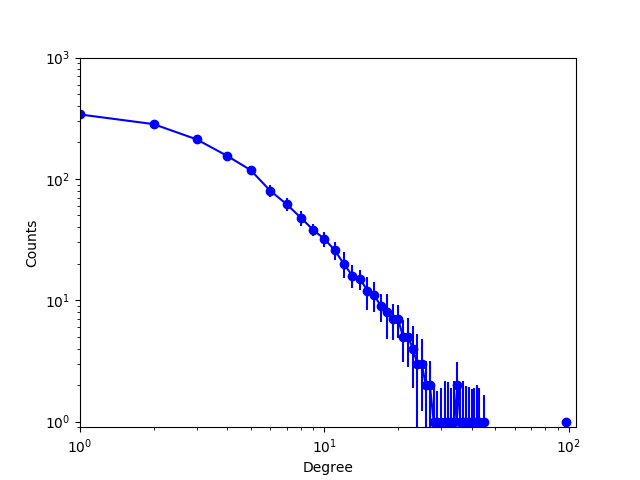
\includegraphics[width=\textwidth]{\lpath/img/corpus/ilfm_protein_0}
            \caption {{\small Protein}}    
            \label{fig:mean and std of net14}
        \end{subfigure}
        %\quad
        %\hfill
        \caption{ILFM global degree distribution in the $M_e$ settings. } 
        \label{fig:me_fit_gburst_ilfm}
\end{figure}


\begin{table}
    \caption{Power law Goodness of fit for the \textbf{global} preferential attachment effect.}
\centering
	\begin{tabular}{@{}lllll@{}}
\toprule

\textbf{IMMSB} & pvalue & alpha & x\_min & n\_tail \\\midrule

Manufacturing & 0.003 \(\pm\) 0.004 & 1.233 \(\pm\) 0.002 & 1.0 \(\pm\) 0.0 & 164.4 \(\pm\) 1.837 \\
UC Irvine & 1.0 \(\pm\) 0.0 & 1.342 \(\pm\) 0.002 & 1.0 \(\pm\) 0.0 & 1845.4 \(\pm\) 7.446 \\
Blogs & 1.0 \(\pm\) 0.0 & 1.336 \(\pm\) 0.002 & 1.0 \(\pm\) 0.0 & 1443.4 \(\pm\) 4.991 \\
Emaileu & 0.0 \(\pm\) 0.0 & 1.362 \(\pm\) 0.044 & 2.567 \(\pm\) 0.667 & 1004.0 \(\pm\) 0.0 \\
Protein & 1.0 \(\pm\) 0.0 & 1.516 \(\pm\) 0.003 & 1.0 \(\pm\) 0.0 & 2062.267 \(\pm\) 6.598 \\
Network 1 & 0.917 \(\pm\) 0.103 & 1.396 \(\pm\) 0.004 & 1.0 \(\pm\) 0.0 & 991.367 \(\pm\) 2.401 \\
Network 2 & 1.0 \(\pm\) 0.0 & 1.447 \(\pm\) 0.004 & 1.0 \(\pm\) 0.0 & 971.933 \(\pm\) 4.396 \\
Network 3 & 0.0 \(\pm\) 0.0 & 1.294 \(\pm\) 0.001 & 1.0 \(\pm\) 0.0 & 998.467 \(\pm\) 1.024 \\
Network 4 & 0.0 \(\pm\) 0.0 & 1.282 \(\pm\) 0.05 & 3.7 \(\pm\) 1.656 & 1000.0 \(\pm\) 0.0 \\

\bottomrule
\end{tabular}

	\begin{tabular}{@{}lllll@{}}
\toprule

\textbf{IBP} & pvalue & alpha & x\_min & n\_tail \\\midrule

Manufacturing & 0.0 \(\pm\) 0.0 & 1.225 \(\pm\) 0.003 & 1.0 \(\pm\) 0.0 & 155.533 \(\pm\) 2.029 \\
UC Irvine & 1.0 \(\pm\) 0.0 & 1.345 \(\pm\) 0.002 & 1.0 \(\pm\) 0.0 & 1784.2 \(\pm\) 8.927 \\
Blogs & 1.0 \(\pm\) 0.0 & 1.336 \(\pm\) 0.002 & 1.0 \(\pm\) 0.0 & 1376.333 \(\pm\) 8.673 \\
Emaileu & 0.024 \(\pm\) 0.027 & 1.257 \(\pm\) 0.001 & 1.0 \(\pm\) 0.0 & 964.467 \(\pm\) 5.194 \\
Protein & 1.0 \(\pm\) 0.0 & 1.572 \(\pm\) 0.006 & 1.0 \(\pm\) 0.0 & 1544.333 \(\pm\) 14.961 \\
Network 1 & 1.0 \(\pm\) 0.0 & 1.408 \(\pm\) 0.003 & 1.0 \(\pm\) 0.0 & 930.0 \(\pm\) 5.727 \\
Network 2 & 1.0 \(\pm\) 0.0 & 1.45 \(\pm\) 0.005 & 1.0 \(\pm\) 0.0 & 897.567 \(\pm\) 7.645 \\
Network 3 & 0.003 \(\pm\) 0.008 & 1.304 \(\pm\) 0.001 & 1.0 \(\pm\) 0.0 & 984.5 \(\pm\) 2.941 \\
Network 4 & 0.0 \(\pm\) 0.0 & 1.199 \(\pm\) 0.01 & 1.033 \(\pm\) 0.18 & 998.633 \(\pm\) 1.11 \\

\bottomrule
\end{tabular}

\label{table:global_gof}
\end{table}



% Local
The local degree distributions of the  networks generated with IMMSB and ILFM are respectively given in Figures \ref{fig:me_fit_lburst_mmsb} and \ref{fig:me_fit_lburst_ibp}. Table \ref{table:local_gof} reports the corresponding goodness of fit evaluation. 
IMMSB complies with the local preferential attachment  for every network, with a p-value equals to 1,  except, in the lesser extent, for Manufacturing* (p-value = 0.55). We can also noticed that the  variance is very small  over the different classes, except again for Manunufacturing*. The instability observed on this network is probably due to its small number of nodes. For ILFM, the fitness decreases from Network 1* to Network 4* varying between 1 and 0.69. Also, the variance of the p-value is high  for the Network 2* , 3*  and 4* and for Manufacturing*.  Moreover, we can observe on Figure \ref{fig:me_fit_lburst_mmsb} that the local degree distributions follow a straight line on a doubly
logarithmic plot for every network generated with IMMSB whereas it is not the case on Figure  \ref{fig:me_fit_lburst_ibp} for the networks generated with ILFM, notably for Network 3*, Network 4* or Manufacturing*.  This confirms our theoretical results according which IMMSB complies with local preferential attachment when ILFM is neutral.
\textbf{Also, the pvalue has high variance for network 2 to 4 and for manufacturing which is correlated with the decay of the global burstiness}
%\underline{Remember  that the pvalue reported here, corresponds to  the average computed over  the classes}.

\textcolor{red}{here comment...} ~\\
\textcolor{red}{x\_min could be removed from table, I explains earlier how I choose it.}


\begin{figure}[h]
        \centering
        \begin{subfigure}[b]{0.300\textwidth}
            \centering
            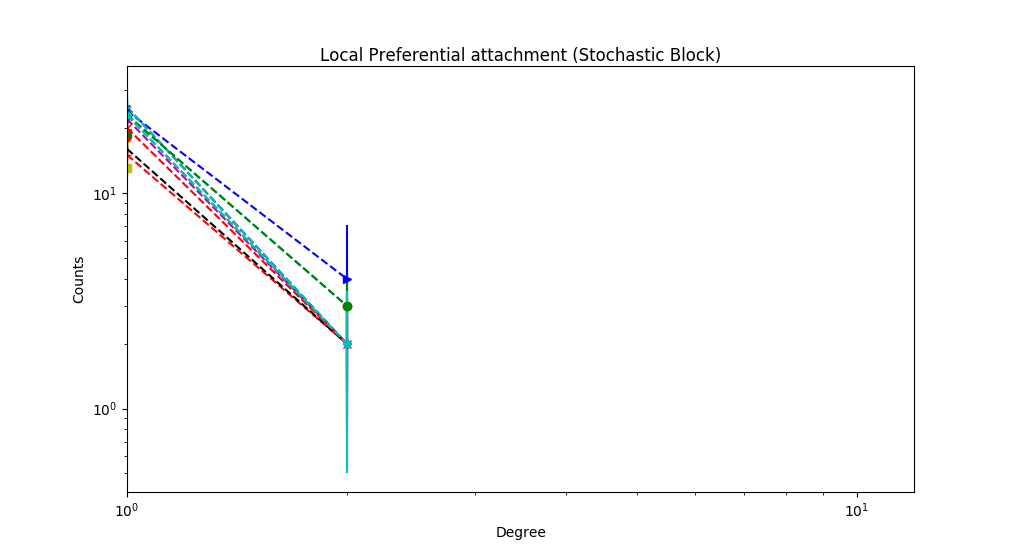
\includegraphics[width=\textwidth]{img/expe/1_mmsb/figure_2}
            \label{fig:mean and std of net14}
            \caption {{\small Network1}}    
        \end{subfigure}
        \begin{subfigure}[b]{0.300\textwidth}
            \centering
            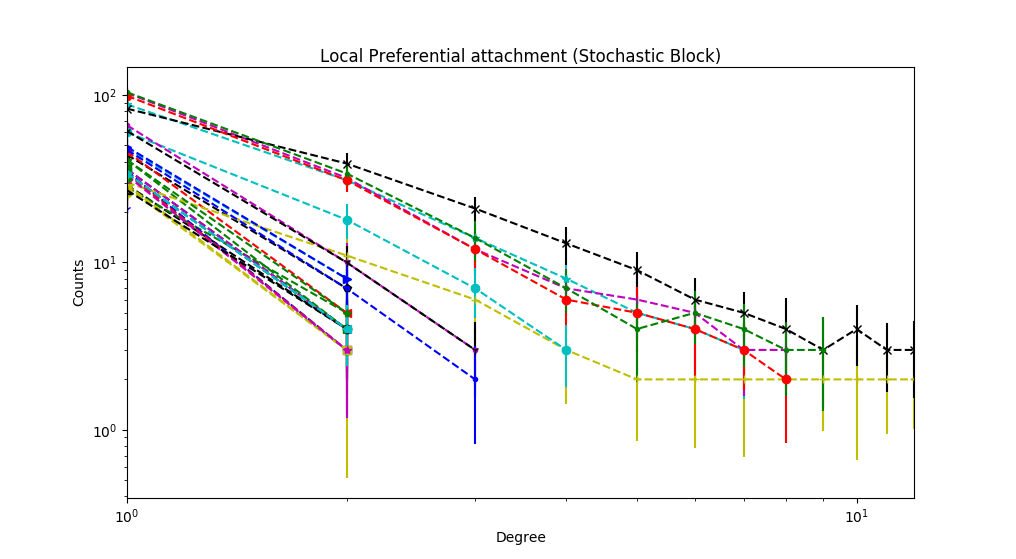
\includegraphics[width=\textwidth]{img/expe/2_mmsb/figure_2}
            \label{fig:mean and std of net14}
            \caption {{\small Network2}}    
        \end{subfigure}
        \begin{subfigure}[b]{0.300\textwidth}
            \centering
            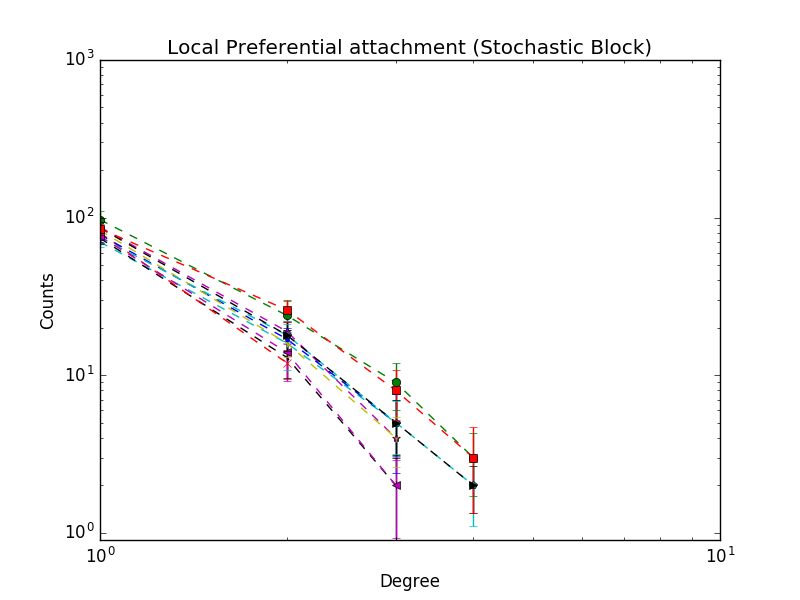
\includegraphics[width=\textwidth]{img/expe/3_mmsb/figure_2}
            \label{fig:mean and std of net14}
            \caption {{\small Network3}}    
        \end{subfigure}
        \begin{subfigure}[b]{0.300\textwidth}
            \centering
            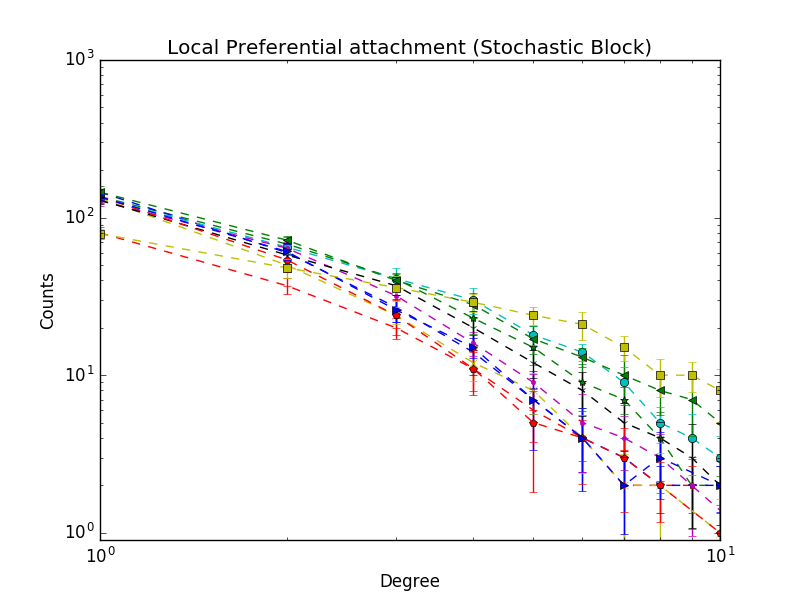
\includegraphics[width=\textwidth]{img/expe/4_mmsb/figure_2}
            \label{fig:mean and std of net14}
            \caption {{\small Network4}}    
        \end{subfigure}
        \begin{subfigure}[b]{0.300\textwidth}
            \centering
            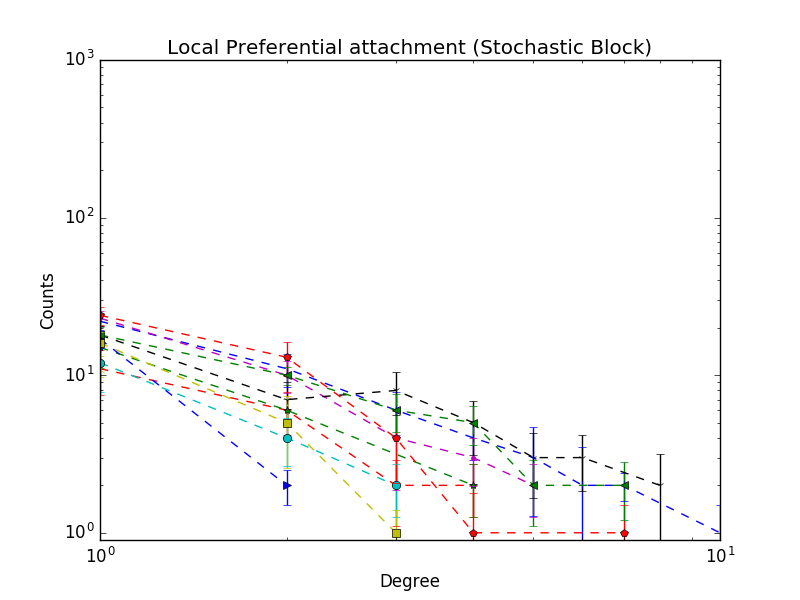
\includegraphics[width=\textwidth]{img/expe/5_mmsb/figure_2}
            \label{fig:mean and std of net14}
            \caption {{\small Manufacturing}}    
        \end{subfigure}
        \begin{subfigure}[b]{0.300\textwidth}
            \centering
            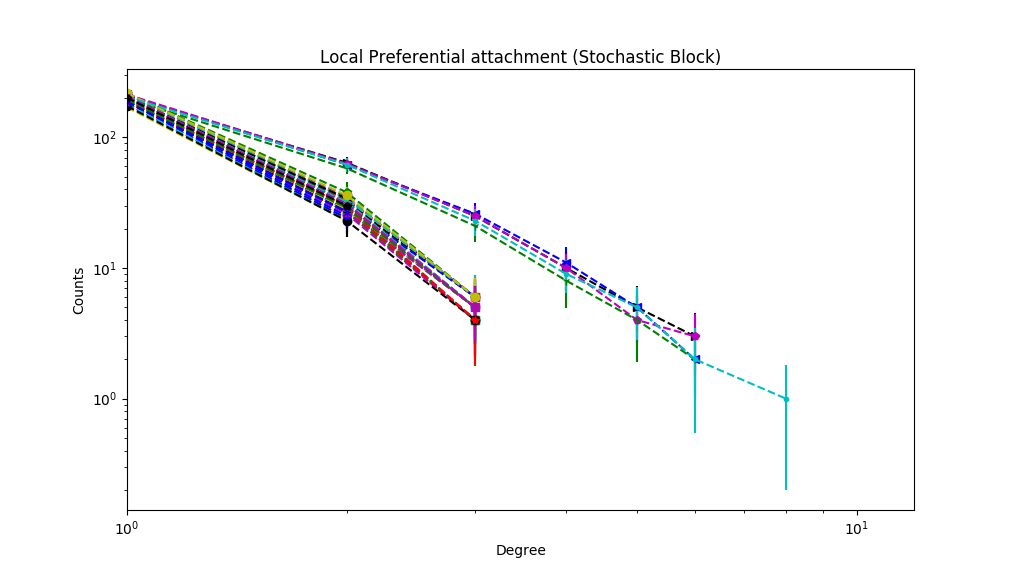
\includegraphics[width=\textwidth]{img/expe/6_mmsb/figure_2}
            \caption {{\small UC Irvine}}    
            \label{fig:mean and std of net14}
        \end{subfigure}
        %\quad
        %\hfill
        \caption{IMMSB Local degree distribution in the $M_e$ settings. } 
\end{figure}


\begin{figure}[h]
        \centering
        \begin{subfigure}[b]{0.300\textwidth}
            \centering
            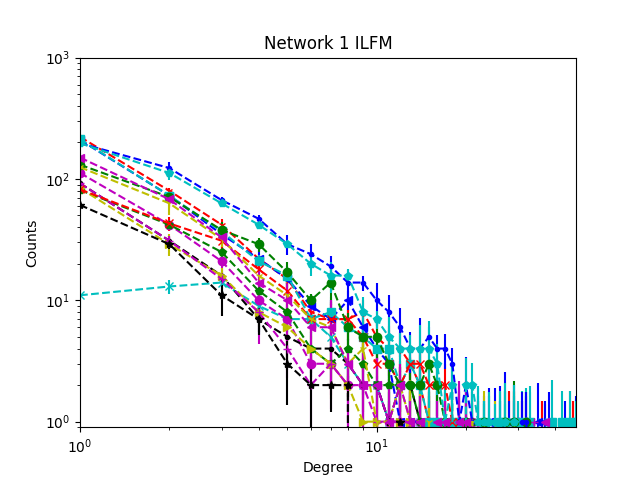
\includegraphics[width=\textwidth]{\lpath/img/corpus/ilfm_network1_1}
            \caption {{\small Network1}}    
        \end{subfigure}
        \begin{subfigure}[b]{0.300\textwidth}
            \centering
            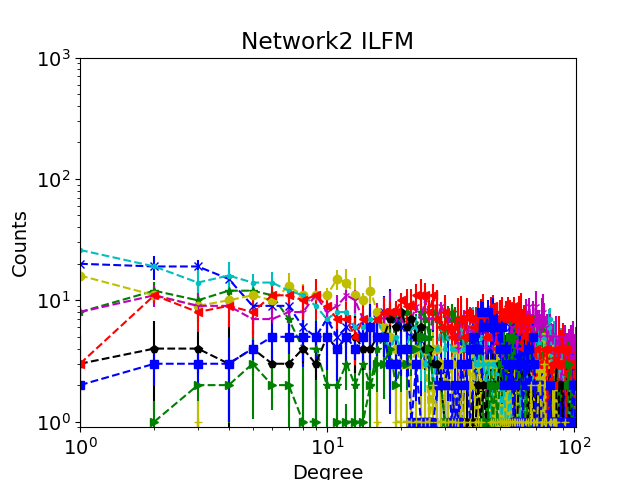
\includegraphics[width=\textwidth]{\lpath/img/corpus/ilfm_network2_1}
            \caption {{\small Network2}}    
        \end{subfigure}
        \begin{subfigure}[b]{0.300\textwidth}
            \centering
            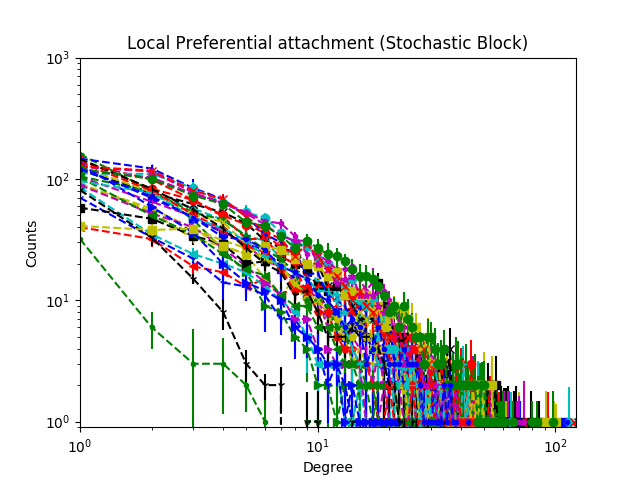
\includegraphics[width=\textwidth]{\lpath/img/corpus/ilfm_network3_1}
            \caption {{\small Network3}}    
        \end{subfigure}
        \begin{subfigure}[b]{0.300\textwidth}
            \centering
            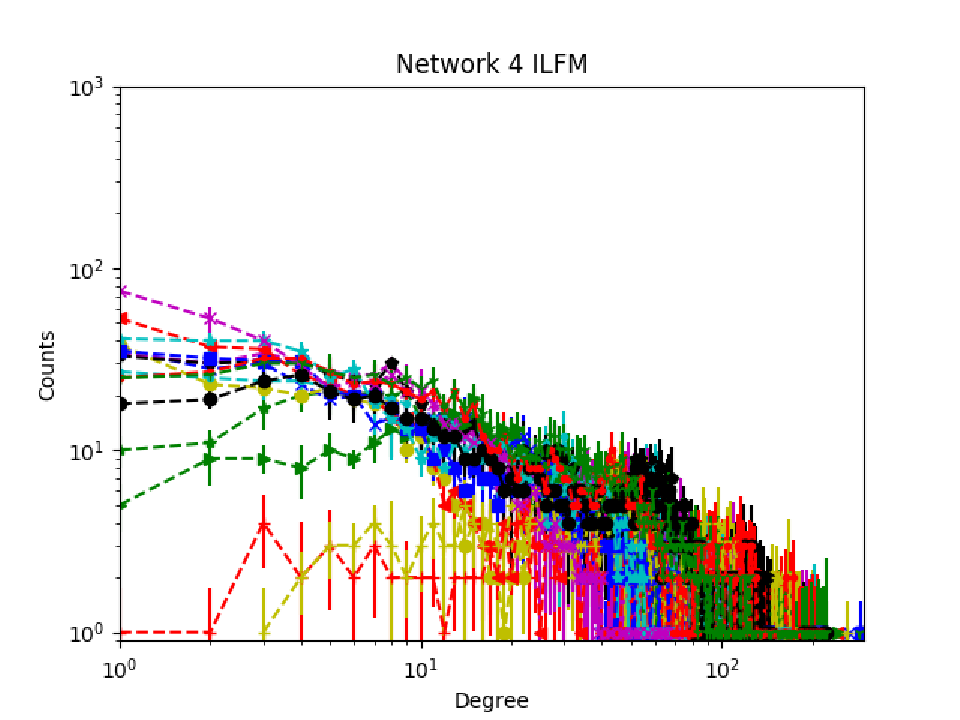
\includegraphics[width=\textwidth]{\lpath/img/corpus/ilfm_network4_1}
            \caption {{\small Network4}}    
        \end{subfigure}
        \begin{subfigure}[b]{0.300\textwidth}
            \centering
            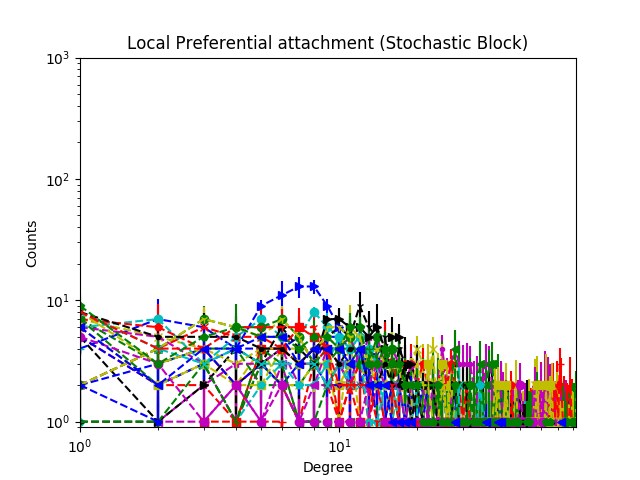
\includegraphics[width=\textwidth]{\lpath/img/corpus/ilfm_manufacturing_1}
            \caption {{\small Manufacturing}}    
        \end{subfigure}
        \begin{subfigure}[b]{0.300\textwidth}
            \centering
            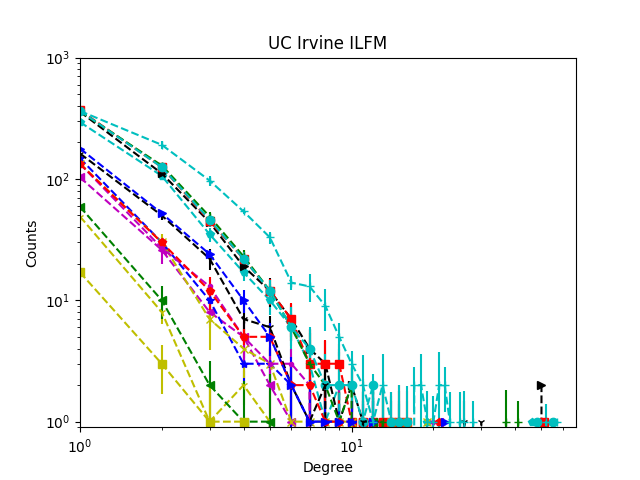
\includegraphics[width=\textwidth]{\lpath/img/corpus/ilfm_ucirvine_1}
            \caption {{\small UC Irvine}}    
            \label{fig:mean and std of net14}
        \end{subfigure}
        \begin{subfigure}[b]{0.300\textwidth}
            \centering
            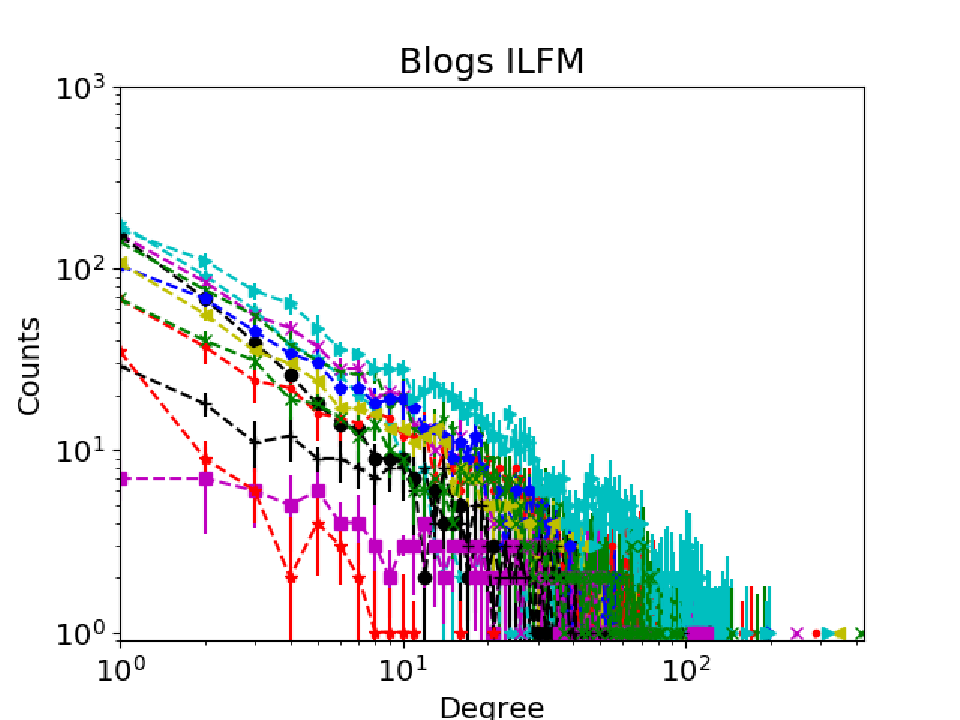
\includegraphics[width=\textwidth]{\lpath/img/corpus/ilfm_blogs_1}
            \caption {{\small Blogs}}    
            \label{fig:mean and std of net14}
        \end{subfigure}
        \begin{subfigure}[b]{0.300\textwidth}
            \centering
            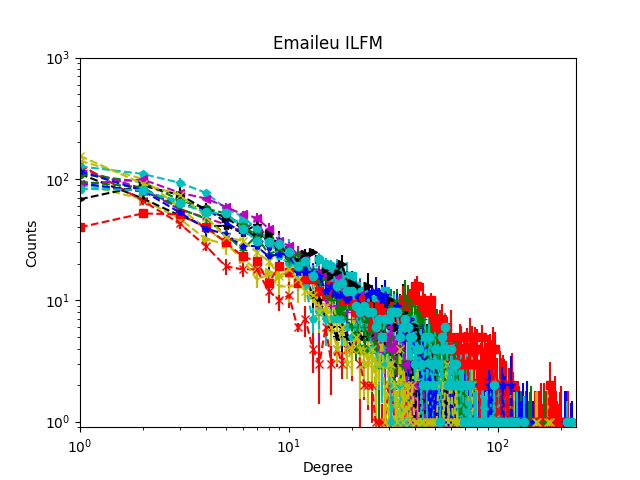
\includegraphics[width=\textwidth]{\lpath/img/corpus/ilfm_emaileu_1}
            \caption {{\small Email Europe}}    
            \label{fig:mean and std of net14}
        \end{subfigure}
        \begin{subfigure}[b]{0.300\textwidth}
            \centering
            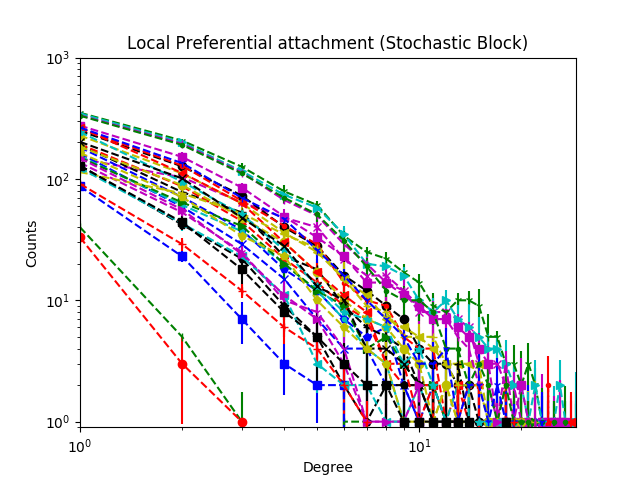
\includegraphics[width=\textwidth]{\lpath/img/corpus/ilfm_protein_1}
            \caption {{\small Protein}}    
            \label{fig:mean and std of net14}
        \end{subfigure}
        %\quad
        %\hfill
        \caption{ILFM Local degree distribution in the $M_e$ settings. } 
        \label{fig:me_fit_lburst_ilfm}
\end{figure}



\begin{table}
    \caption{Power law Goodness of fit for the \textbf{local} preferential attachment effect.}
\centering
	\begin{tabular}{@{}lllll@{}}
\toprule

\textbf{IMMSB} & pvalue & alpha & x\_min & n\_tail \\\midrule

Manufacturing & 0.998 \(\pm\) 0.003 & 1.769 \(\pm\) 0.239 & 1.0 \(\pm\) 0.0 & 42.938 \(\pm\) 10.969 \\
UC Irvine & 1.0 \(\pm\) 0.0 & 3.468 \(\pm\) 1.28 & 1.0 \(\pm\) 0.0 & 348.25 \(\pm\) 98.568 \\
Blogs & 1.0 \(\pm\) 0.0 & 4.462 \(\pm\) 0.923 & 1.0 \(\pm\) 0.0 & 212.533 \(\pm\) 60.408 \\
Emaileu & 1.0 \(\pm\) 0.0 & 3.193 \(\pm\) 0.971 & 1.0 \(\pm\) 0.0 & 335.304 \(\pm\) 111.983 \\
Protein & None \(\pm\) None & None \(\pm\) None & None \(\pm\) None & None \(\pm\) None \\
Network 1 & 1.0 \(\pm\) 0.0 & 2.912 \(\pm\) 1.376 & 1.0 \(\pm\) 0.0 & 145.467 \(\pm\) 68.895 \\
Network 2 & 0.999 \(\pm\) 0.002 & 3.21 \(\pm\) 1.259 & 1.0 \(\pm\) 0.0 & 109.75 \(\pm\) 54.661 \\
Network 3 & 1.0 \(\pm\) 0.0 & 2.637 \(\pm\) 0.584 & 1.0 \(\pm\) 0.0 & 173.667 \(\pm\) 38.348 \\
Network 4 & 1.0 \(\pm\) 0.0 & 1.751 \(\pm\) 0.207 & 1.0 \(\pm\) 0.0 & 357.516 \(\pm\) 76.535 \\

\bottomrule
\end{tabular}

	\begin{tabular}{@{}lllll@{}}
\toprule

\textbf{IBP} & pvalue & alpha & x\_min & n\_tail \\\midrule

Manufacturing & 0.281 \(\pm\) 0.28 & 1.317 \(\pm\) 0.037 & 1.0 \(\pm\)
0.0 & 87.214 \(\pm\) 23.928 \\
UC Irvine & 1.0 \(\pm\) 0.0 & 2.196 \(\pm\) 0.651 & 1.0 \(\pm\)
0.0 & 638.067 \(\pm\) 455.146 \\
Blogs & 1.0 \(\pm\) 0.0 & 1.539 \(\pm\) 0.097 & 1.0 \(\pm\)
0.0 & 897.387 \(\pm\) 244.461 \\
Emaileu & 0.997 \(\pm\) 0.013 & 1.459 \(\pm\) 0.137 & 1.0 \(\pm\)
0.0 & 500.452 \(\pm\) 201.175 \\
Protein & 1.0 \(\pm\) 0.0 & 2.069 \(\pm\) 0.285 & 1.0 \(\pm\)
0.0 & 454.517 \(\pm\) 236.895 \\
Network 1 & 1.0 \(\pm\) 0.0 & 1.808 \(\pm\) 0.307 & 1.0 \(\pm\)
0.0 & 460.355 \(\pm\) 228.692 \\
Network 2 & 1.0 \(\pm\) 0.0 & 1.828 \(\pm\) 0.223 & 1.0 \(\pm\)
0.0 & 412.613 \(\pm\) 206.685 \\
Network 3 & 1.0 \(\pm\) 0.0 & 1.598 \(\pm\) 0.211 & 1.0 \(\pm\)
0.0 & 482.548 \(\pm\) 199.22 \\
Network 4 & 0.499 \(\pm\) 0.474 & 1.311 \(\pm\) 0.098 & 1.0 \(\pm\)
0.0 & 640.677 \(\pm\) 183.136 \\

\bottomrule
\end{tabular}

\label{table:local_gof}
\end{table}

%\subsubsection{Comments}
%
%\begin{itemize}
%    \item global preferential attachment : both IMMSB and ILFM pass the goodness of fit test for networks 1,2 and UC irvine. The 3 other are rejected. This show that the models can fit to strongly bursty networks. When burstiness is less strong, as for network3, we can notice if we consider the tail of the generated distributions, ILFM appears to have straight tail than ILFM.
%    \item local preferential attachment : We can see that the fitness for the local degree distributions of IMMSB is strong for every networks except in the lesser extent for Manufacturing. The confident is also relatively high because of a very small variance over the different class, except again for manunufacturing. The instability of Manufacturing is probably due to his small number of nodes. For ILFM, the fitness decrease from network1 to network4. Also, the pvalue has high variance for network 2 to 4 and for manufacturing which is correlated with the decay of the global burstiness.
%\end{itemize}

\subsection{Homophily}

We evaluate in this section the behaviour of models concerning the homophily effect according to  the natural and the latent similarities.

Table \ref{table:homo_pearson} presents the Pearson correlation coefficient between the probability of having a link $P(y_{ij}=1)$ in the networks generated respectively with ILFM and with IMMSB  and the latent similarity $s_l(i,j)$. Notice that, for the both models, this coefficient  is always equal to one for the natural similarity whereas it takes low values for the latent similarity, always below 0.386, confirming that the both models are neutral for the latent homophily.


In table \ref{table:homo_pearson} we compute the Pearson correlation for the homophily measure. Note that this coefficient for the natural similarity is always equal to one.

We present also in tables \ref{table:homo_natural} and \ref{table:homo_latent} the means and variances of the natural and latent similarities ($s_n(i,j)$ and $s_l(i,j)$) computed on the linked and non-linked pairs of nodes. We can observed that for the both models,  linked nodes are more similar , in average, than non linked nodes in every network for the natural similarity (\ref{table:homo_natural})  whereas for the latent similarityt, we can not observe a  difference between the linked nodes and not linked nodes for the both models. This confirms our theoretical result according which ILFM and IMMSB are homophilic with respect to the natural similarity but not homophilic for the latent similarity

\begin{table}
    \caption{Contingency table for the homophily effect with regards to the choice on the similarity (natural/latent).}
\centering
\begin{tabular}{@{}lllll@{}}
\toprule

\textbf{IMMSB} & natural & latent & natural & latent \\\midrule

Manufacturing & 0.565 \(\pm\) 0.003 & 0.147 \(\pm\) 0.001 & 0.075
\(\pm\) 0.001 & 0.03 \(\pm\) 0.0 \\
UC Irvine & 0.05 \(\pm\) 0.0 & 0.116 \(\pm\) 0.0 & 0.005 \(\pm\)
0.0 & 0.003 \(\pm\) 0.0 \\
Blogs & 0.074 \(\pm\) 0.0 & 0.131 \(\pm\) 0.0 & 0.007 \(\pm\)
0.0 & 0.005 \(\pm\) 0.0 \\
Emaileu & 0.088 \(\pm\) 0.0 & 0.136 \(\pm\) 0.0 & 0.009 \(\pm\)
0.0 & 0.006 \(\pm\) 0.0 \\
Protein & 0.001 \(\pm\) 0.0 & 0.101 \(\pm\) 0.0 & 0.0 \(\pm\) 0.0 & 0.0
\(\pm\) 0.0 \\
Network 1 & 0.049 \(\pm\) 0.001 & 0.124 \(\pm\) 0.002 & 0.006 \(\pm\)
0.0 & 0.037 \(\pm\) 0.001 \\
Network 2 & 0.054 \(\pm\) 0.001 & 0.139 \(\pm\) 0.003 & 0.007 \(\pm\)
0.0 & 0.044 \(\pm\) 0.001 \\
Network 3 & 0.044 \(\pm\) 0.0 & 0.109 \(\pm\) 0.001 & 0.003 \(\pm\)
0.0 & 0.017 \(\pm\) 0.0 \\
Network 4 & 0.212 \(\pm\) 0.0 & 0.119 \(\pm\) 0.0 & 0.022 \(\pm\)
0.0 & 0.014 \(\pm\) 0.0 \\
Manufacturing & 0.114 \(\pm\) 0.001 & 0.107 \(\pm\) 0.0 & 0.032 \(\pm\)
0.0 & 0.026 \(\pm\) 0.0 \\
UC Irvine & 0.005 \(\pm\) 0.0 & 0.101 \(\pm\) 0.0 & 0.0 \(\pm\)
0.0 & 0.0 \(\pm\) 0.0 \\
Blogs & 0.007 \(\pm\) 0.0 & 0.1 \(\pm\) 0.0 & 0.0 \(\pm\) 0.0 & 0.0
\(\pm\) 0.0 \\
Emaileu & 0.022 \(\pm\) 0.0 & 0.101 \(\pm\) 0.0 & 0.001 \(\pm\)
0.0 & 0.001 \(\pm\) 0.0 \\
Protein & 0.001 \(\pm\) 0.0 & 0.1 \(\pm\) 0.0 & 0.0 \(\pm\) 0.0 & 0.0
\(\pm\) 0.0 \\
Network 1 & 0.005 \(\pm\) 0.0 & 0.103 \(\pm\) 0.0 & 0.0 \(\pm\)
0.0 & 0.016 \(\pm\) 0.0 \\
Network 2 & 0.004 \(\pm\) 0.0 & 0.103 \(\pm\) 0.0 & 0.0 \(\pm\)
0.0 & 0.016 \(\pm\) 0.0 \\
Network 3 & 0.011 \(\pm\) 0.0 & 0.102 \(\pm\) 0.0 & 0.0 \(\pm\)
0.0 & 0.014 \(\pm\) 0.0 \\
Network 4 & 0.066 \(\pm\) 0.0 & 0.099 \(\pm\) 0.0 & 0.008 \(\pm\)
0.0 & 0.012 \(\pm\) 0.0 \\

\bottomrule
\end{tabular}

\begin{tabular}{@{}lllll@{}}
\toprule

\textbf{IBP} & natural & latent & natural & latent \\\midrule

Manufacturing & 1.122 \(\pm\) 0.018 & 2.438 \(\pm\) 0.007 & 5.208
\(\pm\) 0.049 & 1.309 \(\pm\) 0.016 \\
UC Irvine & -2.805 \(\pm\) 0.012 & 3.171 \(\pm\) 0.011 & 2.897 \(\pm\)
0.029 & 1.84 \(\pm\) 0.017 \\
Blogs & -2.116 \(\pm\) 0.01 & 2.269 \(\pm\) 0.008 & 2.891 \(\pm\)
0.027 & 1.577 \(\pm\) 0.016 \\
Emaileu & -1.643 \(\pm\) 0.006 & 2.993 \(\pm\) 0.008 & 2.792 \(\pm\)
0.021 & 1.752 \(\pm\) 0.013 \\
Protein & -1.765 \(\pm\) 0.026 & 3.559 \(\pm\) 0.018 & 4.516 \(\pm\)
0.097 & 2.04 \(\pm\) 0.04 \\
Network 1 & -2.19 \(\pm\) 0.02 & 3.038 \(\pm\) 0.017 & 3.086 \(\pm\)
0.067 & 1.939 \(\pm\) 0.036 \\
Network 2 & -1.349 \(\pm\) 0.021 & 3.157 \(\pm\) 0.016 & 3.31 \(\pm\)
0.068 & 2.106 \(\pm\) 0.037 \\
Network 3 & -2.007 \(\pm\) 0.016 & 3.389 \(\pm\) 0.01 & 3.518 \(\pm\)
0.052 & 1.547 \(\pm\) 0.019 \\
Network 4 & -0.053 \(\pm\) 0.007 & 3.278 \(\pm\) 0.003 & 4.457 \(\pm\)
0.018 & 1.769 \(\pm\) 0.006 \\
Manufacturing & -5.496 \(\pm\) 0.008 & 2.277 \(\pm\) 0.002 & 19.72
\(\pm\) 0.031 & 1.285 \(\pm\) 0.004 \\
UC Irvine & -9.306 \(\pm\) 0.0 & 4.675 \(\pm\) 0.0 & 14.428 \(\pm\)
0.001 & 1.794 \(\pm\) 0.0 \\
Blogs & -10.275 \(\pm\) 0.0 & 3.377 \(\pm\) 0.0 & 22.024 \(\pm\)
0.003 & 1.573 \(\pm\) 0.0 \\
Emaileu & -7.269 \(\pm\) 0.001 & 3.349 \(\pm\) 0.0 & 14.537 \(\pm\)
0.003 & 1.708 \(\pm\) 0.0 \\
Protein & -22.429 \(\pm\) 0.0 & 4.195 \(\pm\) 0.0 & 87.031 \(\pm\)
0.004 & 1.714 \(\pm\) 0.0 \\
Network 1 & -11.947 \(\pm\) 0.001 & 4.382 \(\pm\) 0.0 & 27.341 \(\pm\)
0.004 & 2.069 \(\pm\) 0.0 \\
Network 2 & -17.255 \(\pm\) 0.001 & 4.475 \(\pm\) 0.0 & 58.058 \(\pm\)
0.009 & 2.143 \(\pm\) 0.0 \\
Network 3 & -8.508 \(\pm\) 0.001 & 3.241 \(\pm\) 0.0 & 13.094 \(\pm\)
0.003 & 1.271 \(\pm\) 0.0 \\
Network 4 & -6.201 \(\pm\) 0.001 & 2.98 \(\pm\) 0.0 & 9.017 \(\pm\)
0.004 & 1.755 \(\pm\) 0.0 \\

\bottomrule
\end{tabular}

    \label{table:homo_contingency}
\end{table}

\begin{table}[h]
    \caption{Correlation between the latent similarity matrix and the predictive likelihood for IMMSB and ILFM.}
    \centering
    \begin{tabular}{@{}lcc@{}}
\toprule

\textbf{IMMSB} & \textbf{ILFM} \\\midrule

Manufacturing & 0.005 \(\pm\) 0.026 & 0.003 \(\pm\) 0.014 \\
UC Irvine & 0.01 \(\pm\) 0.053 & -0.008 \(\pm\) 0.045 \\
Blogs & 0.019 \(\pm\) 0.101 & -0.006 \(\pm\) 0.034 \\
Emaileu & 0.025 \(\pm\) 0.133 & -0.003 \(\pm\) 0.016 \\
Protein & 0.002 \(\pm\) 0.011 & -0.001 \(\pm\) 0.005 \\
Network 1 & 0.002 \(\pm\) 0.01 & -0.005 \(\pm\) 0.029 \\
Network 2 & 0.003 \(\pm\) 0.016 & -0.004 \(\pm\) 0.019 \\
Network 3 & 0.001 \(\pm\) 0.006 & 0.001 \(\pm\) 0.005 \\
Network 4 & 0.004 \(\pm\) 0.023 & 0.004 \(\pm\) 0.023 \\

\bottomrule
\end{tabular}

    \label{table:homo_pearson}
\end{table}


\subsubsection{Comments}
\begin{itemize}
    \item The measure of the natural similarity over links and non links satisfy the homophily effect for IMMSB and ILFM (table \ref{table:homo_natural_ilfm} and \ref{table:homo_latent_immsb}). In the contrary there is no evidence for a correlation between the latent similarity and the link likelihood (table \ref{table:homo_pearson}). 
\end{itemize}


\subsection{Prediction Performance}
\subsection{Prediction Performance}
In order to evaluate the  prediction performance of the models, we built a training set and a testing set from the original datasets. In order to achieve this, we generate a random mask consisting of 20 percent of the size of the adjacency matrix. This mask is used as our testing set, while the 80 remaining percent are used as a training set. The results for the prediction evaluation are reported in  the AUC-ROC measures in figure \ref{fig:auc}. In addition,  table \ref{table:unbalanced} presents local precision, recall and $F_1$ scores.   Notice the experiments have been done with different  values of initialization for the latent feature dimension K, also given in the table.
\textbf{arevoir}
Each prediction results were averaged on 10 repetitions, and results were found to be stable regarding on the random  initialization and the stochastic optimization procedure. 

% Debug 12 / MASK all

% K = 5

\begin{table*}[h] \label{table:unbalanced}
\caption{Predictive Performance on a UnBalanced Testing set}
	\begin{minipage}[h]{0.45\linewidth} 
K = 5\hspace{5pt}
\begin{tabular}{lllll}
\hline
 IMMSB   &   global &   precision &   recall &    K-\ensuremath{>} \\
\hline
 Network1 b/h         &    0.990 &       0.029 &    0.032 & 5.0 $\pm$ 0.0 \\
 Network2 b/-h       &    0.992 &       0.032 &    0.034 & 5.0 $\pm$ 0.0 \\
 Network3 -b/h       &    0.979 &       0.031 &    0.034 & 5.0 $\pm$ 0.0 \\
 Network4 -b/-h       &    0.887 &       0.151 &    0.192 & 5.0 $\pm$ 0.0 \\

\hline
\end{tabular}
\end{minipage}
\hspace{0.8cm}
\begin{minipage}[h]{0.45\linewidth}
\begin{tabular}{lllll}
\hline
  ILFRM & global &   precision &   recall &     K-\ensuremath{>} \\
\hline
 Network1 b/h       &    0.990 &       0.051 &    0.053 & 13.4 $\pm$ 0.8    \\
 Network2 b/-h     &    0.992 &       0.044 &    0.045 & 14.0 $\pm$ 2.0    \\
 Network3 -b/h     &    0.982 &       0.114 &    0.116 & 10.0 $\pm$ 2.1 \\
 Network4 -b/-h     &    0.926 &       0.389 &    0.393 & 7.2 $\pm$ 1.6     \\

\hline
\end{tabular}
\end{minipage}

% K = 10

	\begin{minipage}[h]{0.45\linewidth} 
K = 10
\begin{tabular}{lllll}
Network1 b/h         &    0.990 &       0.044 &    0.046 & 10.0 $\pm$ 0.0 \\
 Network2 b/-h       &    0.992 &       0.039 &    0.045 & 10.0 $\pm$ 0.0 \\
 Network3 -b/h       &    0.979 &       0.030 &    0.035 & 10.0 $\pm$ 0.0 \\
 Network4 -b/-h       &    0.897 &       0.202 &    0.238 & 10.0 $\pm$ 0.0 \\

\hline
\end{tabular}
\end{minipage}
\hspace{0.8cm}
\begin{minipage}[h]{0.45\linewidth}
\begin{tabular}{lllll}
 Network1 b/h       &    0.990 &       0.049 &    0.053 & 17.2 $\pm$ 2.8 \\
 Network2 b/-h     &    0.992 &       0.047 &    0.051 & 17.2 $\pm$ 2.1 \\
 Network3 -b/h     &    0.982 &       0.132 &    0.132 & 12.2 $\pm$ 2.0 \\
 Network4 -b/-h     &    0.934 &       0.448 &    0.447 & 9.2 $\pm$ 1.2 \\

\hline
\end{tabular}
\end{minipage}

% K = 15

	\begin{minipage}[h]{0.45\linewidth} 
K = 15
\begin{tabular}{lrrrr}
 Network1 b/h         &    0.990 &       0.038 &    0.041 & 15.0 $\pm$ 0.0 \\
 Network2 b/-h       &    0.992 &       0.036 &    0.038 & 15.0 $\pm$ 0.0 \\
 Network3 -b/h       &    0.979 &       0.029 &    0.032 & 15.0 $\pm$ 0.0 \\
 Network4 -b/-h       &    0.898 &       0.207 &    0.245 & 15.0 $\pm$ 0.0 \\

\hline
\end{tabular}
\end{minipage}
\hspace{0.8cm}
\begin{minipage}[h]{0.45\linewidth}
\begin{tabular}{lrrrr}
 Network1 b/h       &    0.990 &       0.050 &    0.053 & 20.6 $\pm$ 2.1 \\
 Network2 b/-h     &    0.992 &       0.049 &    0.055 & 21.2 $\pm$ 2.1 \\
 Network3 -b/h     &    0.983 &       0.164 &    0.166 & 17.2 $\pm$ 1.3 \\
 Network4 -b/-h     &    0.939 &       0.499 &    0.501 & 14.8 $\pm$ 0.4    \\

\hline
\end{tabular}
\end{minipage}

% K = 20

	\begin{minipage}[h]{0.45\linewidth} 
K = 20
\begin{tabular}{lrrrr}

 Network1 b/h          &   0.9899 &      0.0348 &   0.0375 & 20 \\
 Network2 b/-h       &   0.9923 &      0.0494 &   0.0590 & 20 \\
 Network3 -b/-h      &   0.9794 &      0.0289 &   0.0338 & 20 \\
 Network4 -b/h        &   0.9067 &      0.2646 &   0.3034 & 20 \\
\hline
\end{tabular}
\end{minipage}
\hspace{0.8cm}
\begin{minipage}[h]{0.45\linewidth}
\begin{tabular}{lrrrr}
Network1 b/h       &   0.9902 &      0.0641 &   0.0626 &  23 \\
Network2 b/-h     &   0.9915 &      0.0477 &   0.0636 & 17 \\
Network3 -b/h     &   0.9827 &      0.1523 &   0.1518 &  20 \\
Network4 -b/-h     &   0.9396 &      0.4986 &   0.5053 &  22 \\
\hline
\end{tabular}
\end{minipage}
\end{table*}


%%%%%%%%%%%%%%%%%%%%%%%%%%%%%%%%%%%%%%%%%%%%%%%%%%%%%%%%%%%%%%%%%%%%
%%%%%%%%%%%%%%%%%%%%%%%%%%%%%%%%%%%%%%%%%%%%%%%%%%%%%%%%%%%%%%%%%%%%
%%%%%%%%%%%%%%%%%%%%%%%%%%%%%%%%%%%%%%%%%%%%%%%%%%%%%%%%%%%%%%%%%%%%
%%%%%%%%%%%%%%%%%%%%%%%%%%%%%%%%%%%%%%%%%%%%%%%%%%%%%%%%%%%%%%%%%%%%
%%%%%%%%%%%%%%%%%%%%%%%%%%%%%%%%%%%%%%%%%%%%%%%%%%%%%%%%%%%%%%%%%%%%
%%%%%%%%%%%%%%%%%%%%%%%%%%%%%%%%%%%%%%%%%%%%%%%%%%%%%%%%%%%%%%%%%%%%


% Debug 11 / MASK 1

% K = 5

\begin{table*}[h] \label{table:balanced}
\caption{Predictive Performance on a Balanced Testing set}
	\begin{minipage}[h]{0.45\linewidth} 
K =  5\hspace{5pt}
\begin{tabular}{lrlll}
\hline
 IMMSB   &   global &   precision &   recall &    K-\ensuremath{>} \\
\hline
 Network1 b/h          &    0.549 &       0.758 &    0.022 & 5.0 $\pm$ 0.0 \\
 Network2 b/-h        &    0.558 &       0.834 &    0.019 & 5.0 $\pm$ 0.0 \\
 Network3 -b/h        &    0.527 &       0.729 &    0.027 & 5.0 $\pm$ 0.0 \\
 Network4 -b/-h        &    0.557 &       0.743 &    0.162 & 5.0 $\pm$ 0.0 \\

\hline
\end{tabular}
\end{minipage}
\hspace{0.8cm}
\begin{minipage}[h]{0.45\linewidth}
\begin{tabular}{lrlll}
\hline
 ILFRM   &   global &   precision &   recall &     K-\ensuremath{>} \\
\hline
 Network1 b/h        &    0.568 &       0.912 &    0.047 & 13.6 $\pm$ 2.3 \\
 Network2 b/-h      &    0.574 &       0.893 &    0.041 & 16.4 $\pm$ 3.4 \\
 Network3 -b/h      &    0.571 &       0.912 &    0.100 & 9.2 $\pm$ 1.3 \\
 Network4 -b/-h      &    0.668 &       0.906 &    0.362 & 7.6 $\pm$ 1.3 \\

\hline
\end{tabular}
\end{minipage}

% K = 10

	\begin{minipage}[h]{0.45\linewidth} 
K = 10
\begin{tabular}{lrrrr}
 Network1 b/h          &    0.558 &       0.842 &    0.028 & 10.0 $\pm$ 0.0 \\
 Network2 b/-h        &    0.567 &       0.926 &    0.034 & 10.0 $\pm$ 0.0 \\
 Network3 -b/h        &    0.530 &       0.776 &    0.027 & 10.0 $\pm$ 0.0 \\
 Network4 -b/-h        &    0.567 &       0.764 &    0.184 & 10.0 $\pm$ 0.0 \\

\hline
\end{tabular}
\end{minipage}
\hspace{0.8cm}
\begin{minipage}[h]{0.45\linewidth}
\begin{tabular}{lrrrr}
 Network1 b/h        &    0.556 &       0.928 &    0.044 & 17.2 $\pm$ 2.0 \\
 Network2 b/-h      &    0.573 &       0.935 &    0.041 & 17.6 $\pm$ 3.2    \\
 Network3 -b/h      &    0.579 &       0.947 &    0.118 & 12.8 $\pm$ 0.9 \\
 Network4 -b/-h      &    0.718 &       0.943 &    0.457 & 10.8 $\pm$ 0.7 \\

\hline
\end{tabular}
\end{minipage}

% K = 15

	\begin{minipage}[h]{0.45\linewidth} 
K = 15
\begin{tabular}{lrrrr}
 Network1 b/h          &    0.555 &       0.871 &    0.035 & 15.0 $\pm$ 0.0 \\
 Network2 b/-h        &    0.570 &       0.854 &    0.030 & 15.0 $\pm$ 0.0 \\
 Network3 -b/h        &    0.532 &       0.728 &    0.027 & 15.0 $\pm$ 0.0 \\
 Network4 -b/-h        &    0.565 &       0.757 &    0.178 & 15.0 $\pm$ 0.0 \\

\hline
\end{tabular}
\end{minipage}
\hspace{0.8cm}
\begin{minipage}[h]{0.45\linewidth}
\begin{tabular}{lrrrr}
 Network1 b/h        &    0.569 &       0.928 &    0.046 & 20.8 $\pm$ 1.3 \\
 Network2 b/-h      &    0.564 &       0.903 &    0.042 & 21.6 $\pm$ 2.4 \\
 Network3 -b/h      &    0.594 &       0.952 &    0.153 & 18.0 $\pm$ 0.8 \\
 Network4 -b/-h      &    0.723 &       0.945 &    0.467 & 15.0 $\pm$ 0.0    \\

\hline
\end{tabular}
\end{minipage}

% K = 20

	\begin{minipage}[h]{0.45\linewidth} 
K = 20
\begin{tabular}{lrrrr}

 Network1 b/h           &   0.5501 &      0.8980 &   0.0425 & 20 \\
 Network2 b/-h        &   0.5734 &      0.9615 &   0.0326 & 20 \\
 Network3 -b/-h       &   0.5286 &      0.6456 &   0.0255 & 20 \\
 Network4 -b/h         &   0.5577 &      0.7475 &   0.1662 & 20 \\
\hline
\end{tabular}
\end{minipage}
\hspace{0.8cm}
\begin{minipage}[h]{0.45\linewidth}
\begin{tabular}{lrrrr}
 Network1 b/h         &   0.5428 &      0.9737 &   0.0359 &  21 \\
 Network2 b/-h      &   0.5577 &      0.8462 &   0.0389 &  20 \\
 Network3 -b/-h     &   0.5997 &      0.9503 &   0.1630 &  22 \\
 Network4 -b/-h      &   0.7291 &      0.9473 &   0.4813 & 20 \\
\hline
\end{tabular}
\end{minipage}
\end{table*}




\begin{figure}[h]
        \centering
        \begin{subfigure}[b]{0.300\textwidth}
            \centering
            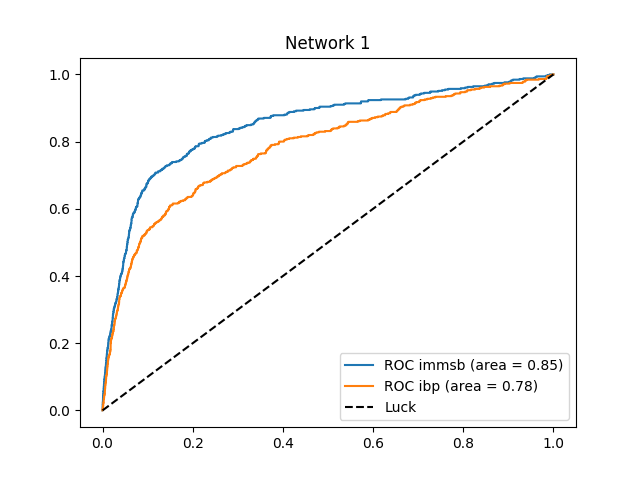
\includegraphics[width=\textwidth]{img/corpus/roc_network1}
            \label{fig:mean and std of net14}
            \caption {{\small Network1}}    
        \end{subfigure}
        \begin{subfigure}[b]{0.300\textwidth}
            \centering
            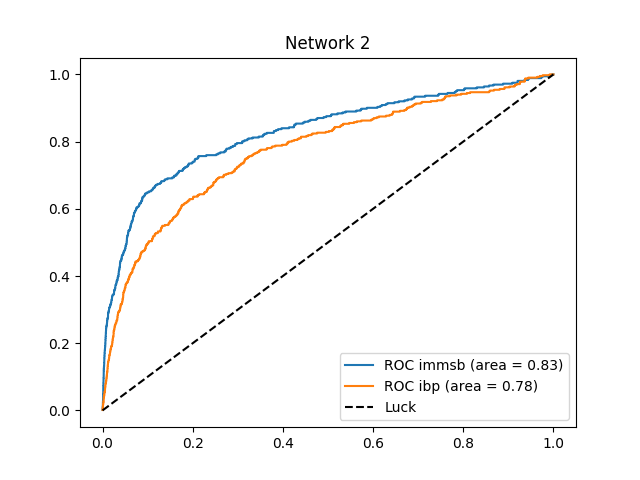
\includegraphics[width=\textwidth]{img/corpus/roc_network2}
            \label{fig:mean and std of net14}
            \caption {{\small Network2}}    
        \end{subfigure}
        \begin{subfigure}[b]{0.300\textwidth}
            \centering
            \includegraphics[width=\textwidth]{img/corpus/roc_network3}
            \label{fig:mean and std of net14}
            \caption {{\small Network3}}    
        \end{subfigure}
        \begin{subfigure}[b]{0.300\textwidth}
            \centering
            \includegraphics[width=\textwidth]{img/corpus/roc_network4}
            \label{fig:mean and std of net14}
            \caption {{\small Network4}}    
        \end{subfigure}
        \begin{subfigure}[b]{0.300\textwidth}
            \centering
            \includegraphics[width=\textwidth]{img/corpus/roc_manufacturing}
            \label{fig:mean and std of net14}
            \caption {{\small Manufacturing}}    
        \end{subfigure}
        \begin{subfigure}[b]{0.300\textwidth}
            \centering
            \includegraphics[width=\textwidth]{img/corpus/roc_ucirvine}
            \label{fig:mean and std of net14}
            \caption {{\small Manufacturing}}    
        \end{subfigure}
        \begin{subfigure}[b]{0.300\textwidth}
            \centering
            \includegraphics[width=\textwidth]{img/corpus/roc_blogs}
            \caption {{\small Blogs}}    
            \label{fig:mean and std of net14}
        \end{subfigure}
        \begin{subfigure}[b]{0.300\textwidth}
            \centering
            \includegraphics[width=\textwidth]{img/corpus/roc_emaileu}
            \caption {{\small Email Europe}}    
            \label{fig:mean and std of net14}
        \end{subfigure}
        \begin{subfigure}[b]{0.300\textwidth}
            \centering
            \includegraphics[width=\textwidth]{img/corpus/roc_protein}
            \caption {{\small Protein}}    
            \label{fig:mean and std of net14}
        \end{subfigure}
        %\quad
        %\hfill
	\caption{AUC curves that compare the performance of ILFM and IMMSB on the 4 synthetic networks.}
	\label{fig:auc}
\end{figure}


\subsubsection{Comments}

\begin{itemize}
\item comparing the performance between both models in the links prediction precision and recall and $F_1$ measure (ref{table:unbalanced}), can seem to conflict with results in the ROC curve (\ref{fig:auc}). More precisely we see that ILFM dominate IMMSB on the $f_1$ measures on all experiments except for one (network 1, K=15). But on the AUC-ROC analysis( \ref{fig:auc}) we see that IMMSB dominate ILFM for two networks (Networks 1 and Networks 2), although it's number of latent feature is almost half lesser than for ILFM. This behavior is also reflected on the accuracy for both models (global precision); The accuracy of IMMSB models is higher for the Network1 and Network2, and this is the opposite for ILFM, which are more accurate for Network3 and Network4. Interestingly, we see that for ILFM, the dimension of the latent feature for which ILFM converged, for the two first networks is significantly higher than the two other. In other words the ILFM model seems to compensate is weak performance by increasing the number of features.
 
\end{itemize}

%\section{$M_e$ -- Model Generated}


\bibliographystyle{unsrt}
\bibliography{./a}

\end{document}
